%
% Draft  document skinspace.tex
% Looks at how follicle development may affect expansion of the skin
%
 
\documentclass[titlepage]{article}  % Latex2e
\usepackage{graphicx,lscape,subfigure}
\usepackage{tikz}
\usepackage{bm,longtable}
\usepackage{textcomp}
 

\title{Does follicle development affect the spatial layout of sheep skin?}
\author{Neville Jackson and Jim Watts}
\date{7 Mar 2018} 

 
\begin{document} 


 
\maketitle      
\tableofcontents

$\newcommand{\E}{\mathrm{E}}$
$\newcommand{\Var}{\mathrm{Var}}$
$\newcommand{\Cov}{\mathrm{Cov}}$ 
$\newcommand{\SD}{\mathrm{SD}}$ 

\clearpage
\section{Introduction} 
 An attempt was made , in Jackson and Watts(2017)~\cite{jack:17b} to put forward the hypothesis that wrinkles form in the foetus at the same stage as secondary follicle development so would be likely to affect secondary follicle density or S/P ratio or secondary fibre diameter. This was based on a somewhat obsure reference (Bogolyubsky (1940)~\cite{bogo:40}) which asserts that wrinkles were observed forming in foetal skin of Karakul and Merino lambs at around 100 days of gestation. There are no other studies of wrinkle development, but there is a considerable literature on follicle development ( see Fraser and Short(1960)~\cite{fras:60} and Maddocks and Jackson(1988)~\cite{madd:88} and Ryder and Stevenson(1968)~\cite{ryde:68} for reviews). There is some literature on collagen development in sheep skin, and we will look at that below.

In Watts and Jackson(2017) and attempt was made to measure collagen type and content, and to relate it to follicle development and to wrinkle development. The study showed that soft, pliable skins with high compressibility had little or no wrinkle development , high follicle densities, fine secondary fibres, less curved follicles, less uneven follicles, and less uneven secondary fibres It was suggested taht there were two mechanisms involved
\begin{itemize}
\item a tradeoff relationship between fibroblast development and follicle development
\item a mechanical interference of collagen fibrils with follicle shape and arrangement.
\end{itemize}.
It was not clear exactly what the mechanism was behind the relationship of compressibility to wrinkle. It was noted that dissection of layer 4 away from the dermis resulted in the wrinkles flattening out - so wrinkle is clearly an excess growth of dermis over that of layer 4, combined with an attachment of the dermis to layer 4.

What we investigate here is the suggestion that it is the follicle development which causes the dermis to expand at a greater rate than layer4



\section{The follicle development - dermal expansion hypothesis}
We noted above that wrinkle development and follicle development occur at the same time in the developing foetal lamb - at about 100days. Wrinkles are certainly visually obvious at birth, and so are follicles because we can see the growing fibres in the birthcoat.

It is one thing to say that because they occur together, wrinkles might affect follicle development. It is another thing to say, as we do here, that it is the other way around - that the growth and development of follicle tissue in the dermis is what causes the dermis to expand at a greater rate than the adjoining layer 4. That extra dermal expansion will not necessarily result in wrinkle - if layer 4 is tightly bound to the lower dermis ( presumably by excessive collagen formation) then the dermis will have to fold as it expands, but if the dermis is only loosely bound to layer 4, it can expand without folding .

So if that is how it works, why do only Merino ( and Merino derived) sheep have wrinkle? Because only Merino sheep have the vastly greater development of secondary follicles with consequent higher S/P ratio and follicle branching.  In all non-Merino breeds the amount of follicle tissue laid down during secondary follicle development is not sufficient to expand the dermis enough to cause it to fold. 

So if SRS-Merino has an even higher S/P ratio then normal Merinos, how is it that they do not develop even more skin folds? Because they also have 'loose' skin - that is skin in which the dermis is not tightly bound to layer 4, but is free to detach and move. The involvement of collagen amount and type in this 'looseness' is conjecture at this stage, but is supported by Watts and Jackson(2017)~\cite{watt:17b}

There is another clue in the fact that skin folds occur in a pattern over the body of a sheep. On the side of the sheep the folds run in a dorso-ventral direction. This corresponds to the direction in which rows of follicle groups run. What we call the E-W direction on an horizontal skin section corresponds to the dorso-ventral direction on the sheep. The rows of follicle groups run parallel to the folds of skin in a sheep with folds. The rows of follicle groups run parallel to the 'laneways' in a sheep without folds. It is clear what is happening. The downgrowths of follicle tissue into the dermis occur in rows ( because the follicle groups are in rows), so they push the dermis aside in rows as they make space to grow. If the dermis is going to expand and fold, it will fold in rows. If the dermis is going to just expand, because it is not bound to the subdermal tissue, there will occur rows of dermis pushed aside by the growing rows of follicles, and we will get 'laneways'. This is not proof, but it is very suggestive that secondary follicle development is involved in wrinkle formation, especially the branching secondary follicles as these are confined to close proximity to the follicle groups. One might object that skin folds are on a larger scale than rows of follicle groups. The answer is that scale does not matter - any sideways expansion will cumulate up to the larger scale of a fold.

There is one contrary piece of evidence. Carter(1943)~\cite{cart:43} states that follicle groups start out in an orderly pattern in the lamb, but the pattern tends to disrupt as the sheep matures. Carter attributes this disruption to collagen growth affecting the follicle arrangement. We are saying here that follicle growth moves the collagen around, at least while the follicles are initiating. Perhaps both occur. Carter links excessive connective tissue growth with formation of wrinkles and folds. That is not necessarily incompatable with what we are proposing here, if connective tissue growth binds the dermis to the subdermal layers.

\section{Materials and Methods}
To investigate  the 'follicles cause dermal expansion' hypothesis, we need a measure of the amount of follicle tissue in skin.
We start by noting that the diameter of a follicle stem at sebacious gland level is close to 3 times the diameter of the fibre it contains. So the area of follicle tissue per $mm^{2}$ at that level is
\begin{displaymath}
F_{a} = 10^{-6} F_{n} \pi \left[\frac{3D}{2}\right]^{2}
\end{displaymath}
$F_{a}$ will vary between 0 and 1 and will represent the follicle tissue area in $mm^{2}$ per $mm^{2}$, so it is unitless.

We next note that the average length of follicles is represented by follicle depth (Fd) in $mm$.  So the volume of follicle tissue per $mm^{2}$  of cross section is
\begin{displaymath}
F_{v} = F_{a} Fd
\end{displaymath}
$F_{v}$ will be $mm^{3}$ of follicle tissue per $mm^{2}$ of cross section, so it will be in $mm$.

The most relevant parameter to area expansion of the dermis is $F_{a}$, so we will be concentrating on $F_{a}$. We note that it is at sebacious gland level, so it is just the follicle stems. Accessory glands are not counted in this measure, only follicle walls and the contained fibre.

We note that it is possible to define $F_{a}$ for secondary follicles only, an that this may be the more relevant parameter. We also note that $F_{a}$ is relative to a 1 $mm^{2}$ area of adult skin, that is after the expansion of dermal tissue has occurred.

\subsection{Sheep studied}
We use the Carter(1968)~\cite{cart:68} to look at $F_{a}$ over a range of breeds.

\subsection{Measurements}
The following measurements and scores were available for the Carter(1968)~\cite{cart:68} data
\begin{description}
\item[]
\end{description}

The following measurements and scores were available for the Jackson(2017)~\cite{jack:17a} ab32 and ab20 CSIRO data
\begin{description}
\item[]
\end{description}

The following measurements and scores were available for the collagen dtts and Jackson(2017)~\cite{watt:17b} dataset
\begin{description}
\item[SkinType] visual scores for sheep skin type. Four grades SRS, semi-SRS, flat, and tight, as defined by Watts et al (2017)~\cite{watt:17}.
\item[TST] total skin thickness in mm. Measured with a ruler graduate in 0.1 mm divisions at 3x magnification on the midside skin sample trimmed of wool stuble and subdermal fat. It consists of epidermis, papillary layer, and reticular layer (layers 1 to 3).
\item[CST] compressed skin thickness in mm. Measured on the trimmed sample with a Mitutoyo ballpoint depth guage ( graduated in 0.1 mm divisions) at four sites. Analyses are of the mean CST over 4 sites.
\item[CMP] compressibility as a percentage. Calculated from CST and TST as $CMP = 100(TST-CST)/TST$. Measures the reduction in thickness under compression as a percentage of the uncompressed thickness.
\item[SkinSoft] skin softness score or ease with which the skin bends or buckles. Five grades (1=hard, unable to bend), to (5=supple, bends easily). Assessed by manually bending the trimmed skin sample in two directions ( north-south = across the rows of follicle groups) and (east-west = along the rows of follicle groups).
\item[S/P] ratio of secondary to primary follicle numbers. This ratio is normally used as a measure of secondary follicle density which is independent of skin expansion during growth. Measured on skin sections.
\item[Fn] follicle number per unit area in follicles per $mm^{2}$. Measured on skin sections with a correction for shrinkage during processing
\item[Dp] mean fibre diameter of secondary fibres in $\mu m$. Measured on skin sections.
\item[DpSD] standard deviation of secondary fibre diameters in $\mu m$. Measured on skin sections.
\end{description}


\subsection{Statistical Methods}
Data were imported into the R statistical program~\cite{rprog:13} and analysed using the {\em lm()} function for regressions, and the {\em aov()} function for analysis of variance.

\section{Results}
\subsection{Breed comparisons of amount of follicle tissue per unit area}
\label{sec:breed}

We look at the range of values for $F_{ap}$ and $F_{as}$ over all breeds sampled by Carter(1968)~\cite{cart:68}. These are shown as histograms in Figures~\ref{fig:faphist} and ~\ref{fig:fashist}.
%\documentclass{article}
%\usepackage{graphicx,subfigure}
%\begin{document}

\begin{figure}[!h]
  \centering
   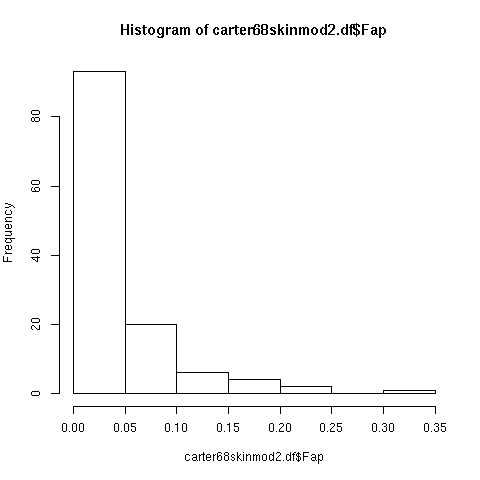
\includegraphics[width=0.9\textwidth]{faphist.png}
%  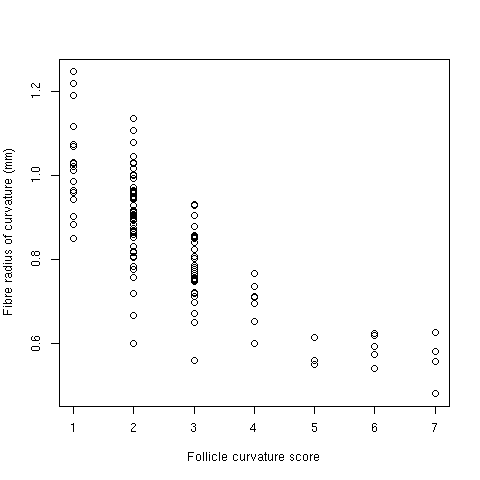
\includegraphics{ofdamm.png}
  \caption{Histogram of breed means for area of primary follicle tissue per $mm^{2}$ of skin at sebaceous gland level from data of Carter(1968)~\cite{cart:68}}
  \label{fig:faphist}
\end{figure}

%\end{document}


%\documentclass{article}
%\usepackage{graphicx,subfigure}
%\begin{document}

\begin{figure}[!h]
  \centering
   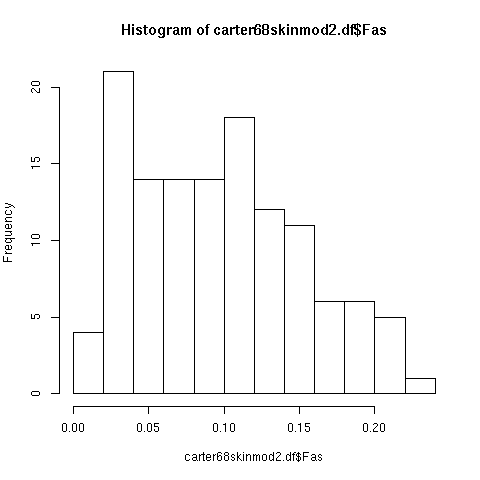
\includegraphics[width=0.9\textwidth]{fashist.png}
%  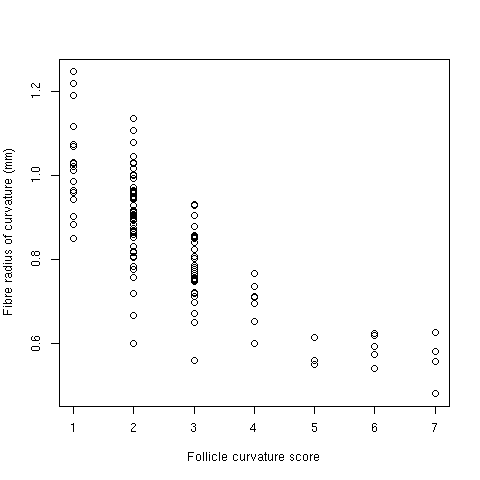
\includegraphics{ofdamm.png}
  \caption{Histogram of breed means for area of secondary follicle tissue per $mm^{2}$ of skin at sebaceous gland level from data of Carter(1968)~\cite{cart:68}}
  \label{fig:fashist}
\end{figure}

%\end{document}


We see a very considerable range in values for both $F_{ap}$ and $F_{as}$. A very small number of breeds have $F_{ap}$ larger than 0.10, whereas many breeds have $F_{as}$ larger than 0.10. 

We need to identify the breeds. This is done in Table~\ref{tab:fabreed}
% latex table generated in R 3.4.2 by xtable 1.8-2 package
% Tue Jan 30 20:57:23 2018
\begin{center}
%\begin{landscape}
\begin{longtable}{|p{1.0in}|p{2.0in}|p{1.0in}|p{1.0in}|}

\caption{Means of Fap and Fas for the Breeds of sheep sampled by Carter(1968)~\cite{cart:68}} \\
\hline
\label{tab:fabreed}
 & Breed & Fap & Fas \\ 
  \hline
1 &  Ak-karaman & 0.02 & 0.03 \\ 
\endfirsthead
\multicolumn{4}{c}%
{\tablename\ \thetable\ -- \textit{Continued from previous page}} \\
\hline
    & Breed  & Fap & Fas  \\ 
\hline
\endhead
\hline
\multicolumn{4}{r}{\textit{Continued on next page}} \\
\endfoot
\hline
\endlastfoot

  2 &  American Merino & 0.01 & 0.09 \\ 
  3 &  American Rambouillet & 0.01 & 0.13 \\ 
  4 &  Arabi & 0.04 & 0.04 \\ 
  5 &  Awassi & 0.04 & 0.04 \\ 
  6 &  Bellari White & 0.19 & 0.02 \\ 
  7 &  Bikaneri & 0.07 & 0.05 \\ 
  8 &  Blackhead Persian & 0.17 & 0.02 \\ 
  9 &  Black Kurumbai Adu & 0.10 & 0.03 \\ 
  10 &  Border Leicester & 0.04 & 0.10 \\ 
  11 &  Cheviot & 0.03 & 0.08 \\ 
  12 &  Chokla & 0.03 & 0.03 \\ 
  13 &  Columbia & 0.01 & 0.11 \\ 
  14 &  Corriedale & 0.02 & 0.15 \\ 
  15 &  Daglic & 0.05 & 0.06 \\ 
  16 &  Debouillet & 0.01 & 0.08 \\ 
  17 &  Dorset Horn & 0.02 & 0.13 \\ 
  18 &  Early Fine Merino & 0.01 & 0.12 \\ 
  19 &  Early Fine Merino (Rambouillet) & 0.01 & 0.13 \\ 
  20 &  English Leicester & 0.03 & 0.11 \\ 
  21 &  German Merinofleischaf & 0.01 & 0.09 \\ 
  22 &  German Merinolandschaf & 0.02 & 0.12 \\ 
  23 &  Icelandic & 0.05 & 0.06 \\ 
  24 &  Ile-de-France & 0.01 & 0.08 \\ 
  25 &  Improved Apulian & 0.01 & 0.08 \\ 
  26 &  Imroz & 0.08 & 0.08 \\ 
  27 &  Ivesi & 0.06 & 0.05 \\ 
  28 &  Jaisalmeri & 0.04 & 0.03 \\ 
  29 &  Kali & 0.04 & 0.03 \\ 
  30 &  Karakaya & 0.07 & 0.05 \\ 
  31 &  Karakul & 0.06 & 0.05 \\ 
  32 &  Kerradi & 0.04 & 0.03 \\ 
  33 &  Kivircik & 0.04 & 0.06 \\ 
  34 &  Limousin & 0.06 & 0.07 \\ 
  35 &  Lincoln & 0.05 & 0.12 \\ 
  36 &  Magra & 0.04 & 0.03 \\ 
  37 &  Malpura & 0.05 & 0.02 \\ 
  38 &  Mandya & 0.30 & 0.04 \\ 
  39 &  Marwari & 0.04 & 0.02 \\ 
  40 &  Merino Tor Mancina & 0.01 & 0.09 \\ 
  41 &  Navajo & 0.02 & 0.08 \\ 
  42 &  Nellore & 0.22 & 0.01 \\ 
  43 &  Nilgiri & 0.03 & 0.07 \\ 
  44 &  Non-Peppin Fine-Medium Merino & 0.01 & 0.15 \\ 
  45 &  Non-Peppin Medium Merino & 0.01 & 0.19 \\ 
  46 &  NSW Fine Merino & 0.01 & 0.17 \\ 
  47 &  Ossimi & 0.05 & 0.13 \\ 
  48 &  Ouda & 0.16 & 0.02 \\ 
  49 &  Peppin Medium Merino & 0.01 & 0.18 \\ 
  50 &  Polwarth & 0.01 & 0.14 \\ 
  51 &  Portuguese Merino & 0.01 & 0.08 \\ 
  52 &  Prealpes du Sud & 0.03 & 0.09 \\ 
  53 &  Rahmani & 0.04 & 0.12 \\ 
  54 &  Romney Marsh & 0.03 & 0.12 \\ 
  55 &  Ryeland & 0.01 & 0.07 \\ 
  56 &  Sakiz & 0.07 & 0.06 \\ 
  57 &  SA Strong Merino & 0.02 & 0.21 \\ 
  58 &  Scottish Blackface & 0.11 & 0.04 \\ 
  59 &  Soay & 0.05 & 0.03 \\ 
  60 &  Sonadi & 0.05 & 0.01 \\ 
  61 &  Sopravissano Rossi & 0.01 & 0.08 \\ 
  62 &  Southdown & 0.02 & 0.12 \\ 
  63 &  Suffolk & 0.02 & 0.06 \\ 
  64 &  Swaledale & 0.12 & 0.04 \\ 
  65 &  Swedish Landrace (Carpet) & 0.08 & 0.10 \\ 
  66 &  Swedish Landrace (Fine) & 0.04 & 0.12 \\ 
  67 &  Tanganyika Long-tailed & 0.13 & 0.01 \\ 
  68 &  Targhee & 0.01 & 0.12 \\ 
  69 &  Tas. Fine Merino & 0.01 & 0.15 \\ 
  70 &  Turkish Merino & 0.01 & 0.08 \\ 
  71 &  Vic. Fine Merino & 0.01 & 0.14 \\ 
  72 &  Welsh Mountain & 0.09 & 0.07 \\ 
  73 &  Wiltshire Horn & 0.07 & 0.08 \\ 
  74 &  Yankasa & 0.21 & 0.03 \\ 
   \hline
\end{longtable}
%\end{landscape}
\end{center}


and we collapse these breeds into Types in Table~\ref{tab:fatype}
% latex table generated in R 3.4.2 by xtable 1.8-2 package
% Tue Jan 30 21:03:37 2018
\begin{table}[ht]
\centering
\caption{Means of Fap and Fas for Types for sheep sampled by Carter(1968)~\cite{cart:68}}
\label{tab:fatype}
\begin{tabular}{rlrr}
  \hline
 & Type & Fap & Fas \\ 
  \hline
1 & African & 0.17 & 0.02 \\ 
  2 & Asian & 0.05 & 0.05 \\ 
  3 & Carpetwool & 0.11 & 0.05 \\ 
  4 & Cheviot & 0.03 & 0.08 \\ 
  5 & Corriedale & 0.02 & 0.15 \\ 
  6 & Downswool & 0.02 & 0.10 \\ 
  7 & Egyptian & 0.04 & 0.13 \\ 
  8 & European & 0.04 & 0.09 \\ 
  9 & Icelandic & 0.05 & 0.06 \\ 
  10 & Indian & 0.09 & 0.03 \\ 
  11 & Longwool & 0.04 & 0.11 \\ 
  12 & Merino & 0.01 & 0.14 \\ 
  13 & Polwarth & 0.01 & 0.14 \\ 
  14 & Soay & 0.05 & 0.03 \\ 
  15 & USA & 0.02 & 0.10 \\ 
  16 & Wiltshire & 0.07 & 0.08 \\ 
   \hline
\end{tabular}
\end{table}


Only the African and Indian hair sheep and the Carpetwools have $F_{ap}$ exceeding 0.10. 
The breeds with $F_{as}$ exceeding 0.10 are the Merino and Merino derived breedsplus the Egyptian  Ossimi and Rahmani. Neither of these Egyptian breeds seem to be wrinkled, but the Merino and its derivatives certainly can be wrinkled.

From these data Fas between 10 and 15 percent seems to be the cutoff point above which dermal expansion is too great and can lead to wrinkle. If the the follicles in a wrinkled sheep are 15-20 percent of the skin area, that means thet the amount of dermal expansion caused by the follicle formation can only be 15-20 percent. That seems a bit small to account for large folds. However, remember that $F_{as}$ is relative to a 1 $mm^{2}$ area after expansion has occurred. To check, we need a measure of dermal expansion. We attempt to develop that in the next section

Before we leave Fas and Fap, we should look at the relation between them. Figure~\ref{fig:fasfap} showns the relationship between means of all 126 flocks sampled by Carter(1968)~\cite{cart:68}.
%\documentclass{article}
%\usepackage{graphicx,subfigure}
%\begin{document}

\begin{figure}[!h]
  \centering
   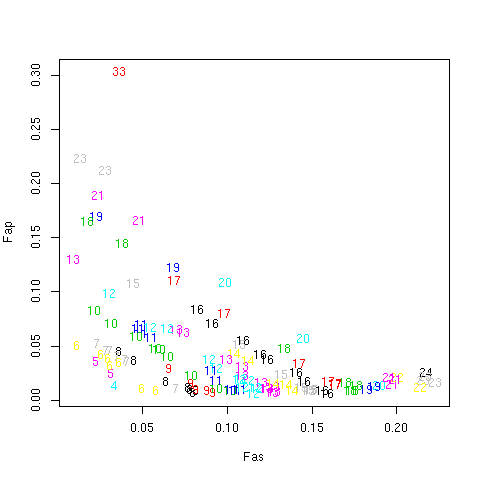
\includegraphics[width=0.9\textwidth]{fasfap.png}
%  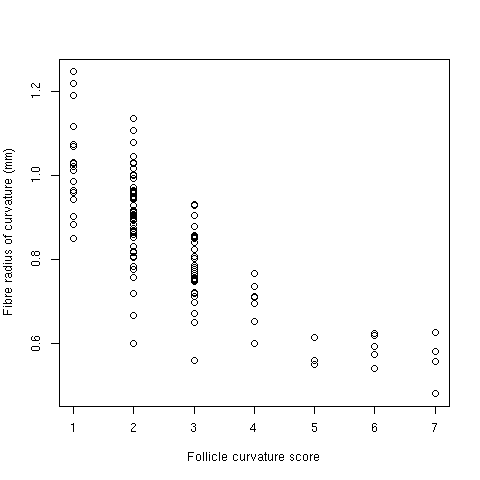
\includegraphics{ofdamm.png}
  \caption{Plot of flock means for area of secondary follicle tissue per $mm^{2}$ of skin against area of primary follicle tissue per $mm^{2}$ of skin for the 126 flocks sampled by Carter(1968)~\cite{cart:68}. The numbers representing each point are the total amount of follicle tissue per $mm^{2}$ of skin as a percentage.}
  \label{fig:fasfap}
\end{figure}

%\end{document}


 It would seem that sheep either have a lot of primary follicle tissue, or a lot of secondary follicle tissue, but not both. It would seem that the limit is about 30 percent of skin area consisting of follicle tissue, and this can be all primaries, nearly all secondaries, or a mixture.  The numbers in the body of the graph (representing Fa for each point as a percentage) show that sheep with a high Fa occur along a curve towards the centre of the graph, while sheep with a low Fa occur in the bottom left corner.  This is a classic demonstration of the pre-papilla cell hypothesis (Moore etal (1998)~\cite{moor:98}). 

\subsection{Using $N_{p}$ as a measure of dermal expansion}
It is often assumed that all sheep have the same density of primary follicles at the time when they initiate, and that subsequent differences in $N_{p}$ per unit area reflect differences in skin growth. Skin growth would include expansion of the dermis during secondary follicle initiation, as proposed here. 

It is therefore of interest to have a look at $N_{p}$ variation in the Carte(1968)~\cite{cart:68} data, and in particular to see if it is lower in breeds which exhibit wrinkle. 

Table~\ref{tab:nptype} shown the means of $N_{p}$ for the sheep type groupings of Carter(1968)~\cite{cart:68} and Table~\ref{tab:npbreed} shows the breed means. 
% latex table generated in R 3.4.2 by xtable 1.8-2 package
% Wed Jan 31 20:44:16 2018
\begin{table}[ht]
\centering
\caption{Means of $N_{p}$ for Types of sheep sampled by Carter(1969)~\cite{cart:68}}
\label{tab:nptype}
\begin{tabular}{rlr}
  \hline
 & Type & Npua \\ 
  \hline
1 & African & 3.40 \\ 
  2 & Asian & 2.37 \\ 
  3 & Carpetwool & 2.52 \\ 
  4 & Cheviot & 2.87 \\ 
  5 & Corriedale & 2.13 \\ 
  6 & Downswool & 3.14 \\ 
  7 & Egyptian & 3.00 \\ 
  8 & European & 2.13 \\ 
  9 & Icelandic & 1.50 \\ 
  10 & Indian & 3.64 \\ 
  11 & Longwool & 2.75 \\ 
  12 & Merino & 2.99 \\ 
  13 & Polwarth & 3.52 \\ 
  14 & Soay & 3.60 \\ 
  15 & USA & 1.87 \\ 
  16 & Wiltshire & 2.70 \\ 
   \hline
\end{tabular}
\end{table}


tex table generated in R 3.4.2 by xtable 1.8-2 package
% Wed Jan 31 20:48:35 2018
\begin{center}
%\begin{landscape}
\begin{longtable}{|p{1.0in}|p{2.0in}|p{1.0in}|}

\caption{Means of Np for the Breeds of sheep sampled by Carter(1968)~\c
ite{cart:68}} \\
\hline
\label{tab:npbreed}
 & Breed & Np  \\ 
  \hline
1 &  Ak-karaman & 1.80 \\
\endfirsthead
\multicolumn{3}{c}%
{\tablename\ \thetable\ -- \textit{Continued from previous page}} \\
\hline
    & Breed  & Np   \\ 
\hline
\endhead
\hline
\multicolumn{3}{r}{\textit{Continued on next page}} \\
\endfoot
\hline
\endlastfoot

  2 &  American Merino & 2.80 \\ 
  3 &  American Rambouillet & 2.40 \\ 
  4 &  Arabi & 2.10 \\ 
  5 &  Awassi & 1.90 \\ 
  6 &  Bellari White & 3.00 \\ 
  7 &  Bikaneri & 6.60 \\ 
  8 &  Blackhead Persian & 3.70 \\ 
  9 &  Black Kurumbai Adu & 3.60 \\ 
  10 &  Border Leicester & 3.00 \\ 
  11 &  Cheviot & 2.87 \\ 
  12 &  Chokla & 3.80 \\ 
  13 &  Columbia & 1.80 \\ 
  14 &  Corriedale & 2.13 \\ 
  15 &  Daglic & 2.90 \\ 
  16 &  Debouillet & 3.00 \\ 
  17 &  Dorset Horn & 2.90 \\ 
  18 &  Early Fine Merino & 4.00 \\ 
  19 &  Early Fine Merino (Rambouillet) & 3.45 \\ 
  20 &  English Leicester & 2.50 \\ 
  21 &  German Merinofleischaf & 2.10 \\ 
  22 &  German Merinolandschaf & 2.70 \\ 
  23 &  Icelandic & 1.50 \\ 
  24 &  Ile-de-France & 2.10 \\ 
  25 &  Improved Apulian & 2.30 \\ 
  26 &  Imroz & 3.20 \\ 
  27 &  Ivesi & 2.50 \\ 
  28 &  Jaisalmeri & 3.20 \\ 
  29 &  Kali & 3.10 \\ 
  30 &  Karakaya & 2.10 \\ 
  31 &  Karakul & 3.30 \\ 
  32 &  Kerradi & 1.50 \\ 
  33 &  Kivircik & 2.50 \\ 
  34 &  Limousin & 2.00 \\ 
  35 &  Lincoln & 2.53 \\ 
  36 &  Magra & 3.60 \\ 
  37 &  Malpura & 3.10 \\ 
  38 &  Mandya & 4.70 \\ 
  39 &  Marwari & 3.40 \\ 
  40 &  Merino Tor Mancina & 2.60 \\ 
  41 &  Navajo & 1.80 \\ 
  42 &  Nellore & 2.30 \\ 
  43 &  Nilgiri & 4.10 \\ 
  44 &  Non-Peppin Fine-Medium Merino & 2.25 \\ 
  45 &  Non-Peppin Medium Merino & 2.40 \\ 
  46 &  NSW Fine Merino & 3.40 \\ 
  47 &  Ossimi & 3.00 \\ 
  48 &  Ouda & 3.20 \\ 
  49 &  Peppin Medium Merino & 3.10 \\ 
  50 &  Polwarth & 3.52 \\ 
  51 &  Portuguese Merino & 3.10 \\ 
  52 &  Prealpes du Sud & 2.40 \\ 
  53 &  Rahmani & 3.00 \\ 
  54 &  Romney Marsh & 2.95 \\ 
  55 &  Ryeland & 2.10 \\ 
  56 &  Sakiz & 2.80 \\ 
  57 &  SA Strong Merino & 3.27 \\ 
  58 &  Scottish Blackface & 2.17 \\ 
  59 &  Soay & 3.60 \\ 
  60 &  Sonadi & 2.80 \\ 
  61 &  Sopravissano Rossi & 2.40 \\ 
  62 &  Southdown & 3.80 \\ 
  63 &  Suffolk & 3.50 \\ 
  64 &  Swaledale & 2.30 \\ 
  65 &  Swedish Landrace (Carpet) & 2.10 \\ 
  66 &  Swedish Landrace (Fine) & 1.80 \\ 
  67 &  Tanganyika Long-tailed & 3.30 \\ 
  68 &  Targhee & 2.00 \\ 
  69 &  Tas. Fine Merino & 2.96 \\ 
  70 &  Turkish Merino & 2.40 \\ 
  71 &  Vic. Fine Merino & 3.62 \\ 
  72 &  Welsh Mountain & 3.13 \\ 
  73 &  Wiltshire Horn & 2.70 \\ 
  74 &  Yankasa & 3.40 \\ 
   \hline
\end{longtable}
%\end{landscape}
\end{center}

There is no clear result. The Merino means are intermediate. Clearly growth differences are interfering with our attempt to use $N_{p}$ as an indicator of dermal expansion.

\subsection{Data on variation within a wrinkled Merino flock}
We have a set of data in which degree of wrinkle is actually recorded for each sheep as a scores for neck wrinkle and body wrinkle according to the photographic standards of Turner, etal (1953)~\cite{turn:53}. We also have skin histology measurements for these sheep, so we can calculate $F_{ap}$ and $F_{as}$. This flock is the CSIRO experimant known as AB32, for which genetic parameters are reported by Jackson(2017)~\cite{jack:17a}. There is also a summary of the genetic parameter estimates relevant to wrinkle score in Jackson and Watts(2017)~\cite{jack:17b}.

The first thing we note is that if we look at the relationship of individual sheep Fas estimates and wrinkle scores we see nothing interesting. The correlation is near-zero. There is too much noise. The reason we see something with the Carter data above is that we looked at flock means, which were means of around 20 animals. So what we propose to do here is to look at relationships using sire group means.  We actually list all 78 sire group means in Table~\ref{tab:smeans}.
% latex table generated in R 3.4.2 by xtable 1.8-2 package
% Fri Feb  2 21:32:24 2018
\begin{center}
\begin{longtable}{|p{0.6in}|p{0.5in}|p{0.5in}|p{0.5in}|p{0.5in}|p{0.5in}|p{0.5in}|p{0.5in}|p{0.5in}|}
\caption{Sire family means for 8 traits for CSIRO dataset reported by Jackson(2017)~\cite{jack:17b}.}  \\
\hline
\label{tab:smeans}
  SId & Fap & Fas & Fa & WrN & WrB & WrT & Sarea & Fnpua \\
\hline
\endfirsthead
\multicolumn{9}{c}%
{\tablename\ \thetable\ -- \textit{Continued from previous page}} \\
\hline
 SId & Fap & Fas & Fa & WrN & WrB & WrT & Sarea & Fnpua \\
\hline
\endhead
\hline
\multicolumn{9}{r}{\textit{Continued on next page}} \\
\endfoot
\hline
\endlastfoot

  SId & Fap & Fas & Fa & WrN & WrB & WrT & Sarea & Fnpua \\ 
  \hline
 80L1014 & 0.01 & 0.20 & 0.21 & 2.90 & 2.40 & 5.30 & 1.05 & 2.84 \\ 
 80L1041 & 0.01 & 0.23 & 0.24 & 2.47 & 1.79 & 4.26 & 1.09 & 2.72 \\ 
 80L1048 & 0.01 & 0.21 & 0.22 & 2.93 & 2.21 & 5.14 & 1.13 & 2.72 \\ 
 80L1061 & 0.01 & 0.19 & 0.20 & 1.67 & 1.33 & 3.00 & 1.12 & 3.10 \\ 
 80L1088 & 0.02 & 0.20 & 0.21 & 2.39 & 1.93 & 4.32 & 1.08 & 3.44 \\ 
 80L1102 & 0.01 & 0.19 & 0.21 & 2.33 & 1.48 & 3.81 & 1.08 & 3.14 \\ 
 80L1109 & 0.01 & 0.19 & 0.21 & 1.96 & 1.46 & 3.42 & 1.07 & 3.30 \\ 
 80L1133 & 0.01 & 0.19 & 0.20 & 2.18 & 1.55 & 3.73 & 1.07 & 3.72 \\ 
 80L1139 & 0.01 & 0.16 & 0.17 & 2.17 & 1.33 & 3.50 & 1.07 & 3.29 \\ 
 80L1144 & 0.01 & 0.18 & 0.19 & 2.56 & 1.92 & 4.48 & 1.08 & 2.84 \\ 
 80L1157 & 0.02 & 0.20 & 0.22 & 2.50 & 1.67 & 4.17 & 1.01 & 3.31 \\ 
 80L1158 & 0.01 & 0.21 & 0.22 & 1.86 & 1.33 & 3.19 & 1.13 & 3.93 \\ 
 80L1190 & 0.01 & 0.20 & 0.21 & 2.00 & 1.38 & 3.38 & 1.09 & 3.13 \\ 
 80L1212 & 0.01 & 0.17 & 0.18 & 2.29 & 1.65 & 3.94 & 1.05 & 2.87 \\ 
 80L1213 & 0.01 & 0.19 & 0.20 & 2.48 & 1.74 & 4.22 & 1.06 & 2.83 \\ 
 80L1259 & 0.01 & 0.21 & 0.22 & 2.67 & 1.56 & 4.22 & 1.01 & 2.75 \\ 
 80L1264 & 0.01 & 0.18 & 0.19 & 2.33 & 1.67 & 4.00 & 1.02 & 3.16 \\ 
 80L3002 & 0.02 & 0.21 & 0.23 & 2.75 & 2.00 & 4.75 & 1.01 & 3.07 \\ 
 80L3013 & 0.01 & 0.22 & 0.24 & 4.50 & 3.00 & 7.50 & 1.07 & 2.76 \\ 
 80L3034 & 0.01 & 0.19 & 0.21 & 2.50 & 2.00 & 4.50 & 1.03 & 2.62 \\ 
 80L3035 & 0.01 & 0.20 & 0.21 & 2.71 & 1.86 & 4.57 & 1.06 & 3.19 \\ 
 80L3063 & 0.01 & 0.19 & 0.20 & 3.00 & 2.00 & 5.00 & 1.02 & 2.79 \\ 
 80L3130 & 0.01 & 0.21 & 0.22 & 2.75 & 1.75 & 4.50 & 1.08 & 3.09 \\ 
 80L3138 & 0.01 & 0.18 & 0.19 & 2.00 & 1.50 & 3.50 & 1.05 & 2.82 \\ 
 80L3187 & 0.02 & 0.21 & 0.23 & 2.80 & 2.20 & 5.00 & 0.97 & 3.17 \\ 
 80L3215 & 0.01 & 0.21 & 0.22 & 2.00 & 2.00 & 4.00 & 1.01 & 2.50 \\ 
 80L3238 & 0.02 & 0.24 & 0.26 & 3.00 & 2.00 & 5.00 & 0.92 & 3.80 \\ 
 80L3245 & 0.02 & 0.22 & 0.23 & 2.75 & 1.75 & 4.50 & 1.10 & 3.57 \\ 
 80L3251 & 0.02 & 0.22 & 0.24 & 2.00 & 2.00 & 4.00 & 0.98 & 3.79 \\ 
 80L3268 & 0.01 & 0.20 & 0.21 & 2.75 & 1.25 & 4.00 & 1.05 & 3.59 \\ 
 80L3352 & 0.02 & 0.22 & 0.23 & 2.00 & 1.67 & 3.67 & 1.04 & 3.54 \\ 
 80L3372 & 0.01 & 0.21 & 0.22 & 2.67 & 2.00 & 4.67 & 0.96 & 3.23 \\ 
 80L3394 & 0.02 & 0.23 & 0.25 & 2.50 & 1.50 & 4.00 & 1.04 & 3.96 \\ 
 82L2006 & 0.01 & 0.22 & 0.23 & 3.60 & 3.20 & 6.80 & 1.07 & 2.26 \\ 
 82L2036 & 0.01 & 0.21 & 0.22 & 1.86 & 0.86 & 2.71 & 1.04 & 2.97 \\ 
 82L2068 & 0.01 & 0.21 & 0.23 & 2.57 & 2.14 & 4.71 & 1.07 & 2.70 \\ 
 82L2143 & 0.01 & 0.23 & 0.24 & 2.05 & 1.37 & 3.42 & 1.00 & 3.13 \\ 
 82L2148 & 0.01 & 0.22 & 0.22 & 2.40 & 1.60 & 4.00 & 1.05 & 2.66 \\ 
 82L2170 & 0.01 & 0.26 & 0.27 & 2.75 & 1.88 & 4.62 & 0.85 & 4.33 \\ 
 82L2172 & 0.02 & 0.25 & 0.27 & 2.00 & 1.21 & 3.21 & 0.98 & 3.10 \\ 
 82L2248 & 0.01 & 0.22 & 0.23 & 2.00 & 1.50 & 3.50 & 1.03 & 2.62 \\ 
 82L2250 & 0.01 & 0.27 & 0.28 & 3.00 & 1.75 & 4.75 & 1.06 & 2.38 \\ 
 82L2267 & 0.01 & 0.21 & 0.22 & 2.45 & 1.45 & 3.91 & 1.06 & 2.46 \\ 
 82L2288 & 0.01 & 0.25 & 0.26 & 1.62 & 1.12 & 2.75 & 1.10 & 3.03 \\ 
 82L2296 & 0.01 & 0.22 & 0.23 & 2.19 & 1.31 & 3.50 & 1.02 & 2.88 \\ 
 82L4028 & 0.01 & 0.22 & 0.23 & 1.60 & 1.00 & 2.60 & 1.12 & 2.50 \\ 
 83L1014 & 0.01 & 0.22 & 0.24 & 2.17 & 1.39 & 3.56 & 0.93 & 3.52 \\ 
 83L1055 & 0.01 & 0.23 & 0.25 & 2.17 & 1.61 & 3.78 & 0.94 & 3.53 \\ 
 83L1058 & 0.02 & 0.23 & 0.24 & 2.25 & 2.05 & 4.30 & 0.91 & 3.62 \\ 
 83L1087 & 0.02 & 0.20 & 0.22 & 2.83 & 2.33 & 5.17 & 0.87 & 3.43 \\ 
 83L1118 & 0.02 & 0.26 & 0.27 & 2.33 & 1.87 & 4.20 & 0.89 & 3.89 \\ 
 83L1119 & 0.02 & 0.22 & 0.23 & 2.73 & 2.00 & 4.73 & 0.88 & 3.61 \\ 
 83L1143 & 0.02 & 0.20 & 0.22 & 3.10 & 2.30 & 5.40 & 0.90 & 3.51 \\ 
 83L1144 & 0.02 & 0.22 & 0.24 & 2.47 & 2.24 & 4.71 & 0.87 & 3.30 \\ 
 83L1159 & 0.01 & 0.20 & 0.21 & 2.05 & 1.45 & 3.50 & 0.89 & 3.73 \\ 
 83L1199 & 0.02 & 0.23 & 0.25 & 2.43 & 2.14 & 4.57 & 0.91 & 3.53 \\ 
 83L1233 & 0.01 & 0.22 & 0.23 & 1.83 & 1.17 & 3.00 & 0.87 & 3.99 \\ 
 83L1237 & 0.02 & 0.22 & 0.24 & 2.71 & 2.21 & 4.93 & 0.85 & 3.27 \\ 
 83L1253 & 0.01 & 0.20 & 0.22 & 2.55 & 2.00 & 4.55 & 0.91 & 3.53 \\ 
 83L1265 & 0.02 & 0.25 & 0.26 & 3.09 & 2.64 & 5.73 & 0.83 & 3.67 \\ 
 83L3022 & 0.01 & 0.19 & 0.21 & 2.67 & 2.00 & 4.67 & 0.86 & 3.81 \\ 
 83L3026 & 0.01 & 0.22 & 0.23 & 3.50 & 2.00 & 5.50 & 0.81 & 3.87 \\ 
 83L3096 & 0.01 & 0.23 & 0.24 & 4.00 & 3.00 & 7.00 & 0.90 & 3.09 \\ 
 83L3102 & 0.02 & 0.25 & 0.27 & 2.50 & 2.00 & 4.50 & 0.86 & 3.32 \\ 
 83L3144 & 0.02 & 0.22 & 0.24 & 3.75 & 3.00 & 6.75 & 0.86 & 4.13 \\ 
 83L3171 & 0.02 & 0.25 & 0.27 & 3.67 & 2.67 & 6.33 & 0.89 & 3.72 \\ 
 83L3214 & 0.02 & 0.19 & 0.21 & 3.00 & 2.00 & 5.00 & 0.92 & 3.96 \\ 
 83L3222 & 0.02 & 0.22 & 0.24 & 3.43 & 2.71 & 6.14 & 0.90 & 3.81 \\ 
 83L3275 & 0.01 & 0.23 & 0.24 & 2.50 & 2.00 & 4.50 & 0.92 & 3.56 \\ 
 83L3278 & 0.02 & 0.26 & 0.27 & 3.00 & 3.00 & 6.00 & 0.82 & 4.29 \\ 
 83L3294 & 0.03 & 0.16 & 0.19 & 2.00 & 0.00 & 2.00 & 0.84 & 4.03 \\ 
 83L3296 & 0.02 & 0.28 & 0.29 & 3.00 & 2.50 & 5.50 & 0.88 & 4.12 \\ 
 83L3309 & 0.02 & 0.22 & 0.23 & 2.60 & 2.20 & 4.80 & 0.92 & 3.73 \\ 
 83L3346 & 0.02 & 0.24 & 0.25 & 2.00 & 1.50 & 3.50 & 0.84 & 4.02 \\ 
 83L3371 & 0.02 & 0.22 & 0.23 & 2.50 & 2.00 & 4.50 & 0.89 & 3.17 \\ 
 83L3409 & 0.02 & 0.22 & 0.24 & 2.25 & 1.25 & 3.50 & 0.90 & 3.64 \\ 
 83L3458 & 0.01 & 0.23 & 0.24 & 3.00 & 2.00 & 5.00 & 0.79 & 3.95 \\ 
 83L3467 & 0.02 & 0.21 & 0.23 & 2.00 & 1.00 & 3.00 & 0.99 & 3.85 \\ 
   \hline
\end{longtable}
\end{center}
%\end{document}


Relationships among sire group means are a rough way of looking at genetic correlations. We use this approach, rather than a full genetic analysis, because we do not really know what what traits we are interested in yet.

We start by looking at the sire group means correlation of $F_{as}$ with total wrinkle score (WrT). This is shown in Figure~\ref{fig:faswrt}
%\documentclass{article}
%\usepackage{graphicx,subfigure}
%\begin{document}

\begin{figure}[!h]
  \centering
   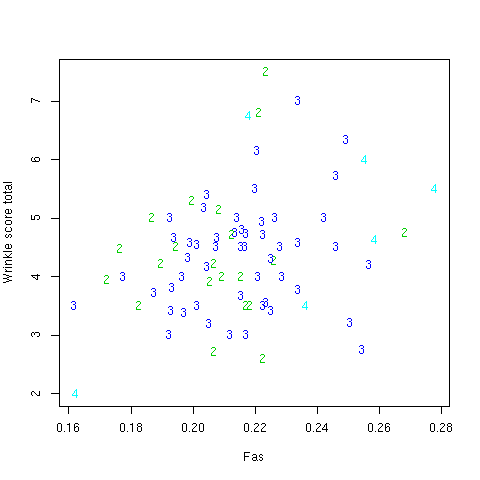
\includegraphics[width=0.9\textwidth]{faswrt.png}
  \caption{Plot of sire group means  of secondary follicle tissue per $mm^{2}$ against total wrinkle score (WrT). The numbers representing each point are $Np$.}
  \label{fig:faswrt}
\end{figure}

%\end{document}


We see a positive correlation of 0.29, which is significant at $P<0.05$ for 74 sire groups.  The numbers labelling each point show that $N_{p}$ does not vary in any consistent way across this graph. We interpret this as follows. $F_{as}$ indicates likely dermal expansion due to secondary follicle development, so we would expect higher dermal expansion to be associated with higher wrinkle scores, and it comes out that way. We do not expect a very strong correlation, because wrinkle formation depends on collagen structure as wella s on follicle induced dermal expansion. $N_{p}$ indicates overall skin expansion, due to overall growth, as well as extra dermal expansion induced by follicle development. We do not expect a strong relationship of $N_{p}$ with wrinkle. 

We next note that the scoring of wrinkle seems to be affected by size of the animal. Figure~\ref{fig:sawrt} shows that sheep with large surface area tend to get a lower wrinkle score.
%\documentclass{article}
%\usepackage{graphicx,subfigure}
%\begin{document}

\begin{figure}[!h]
  \centering
   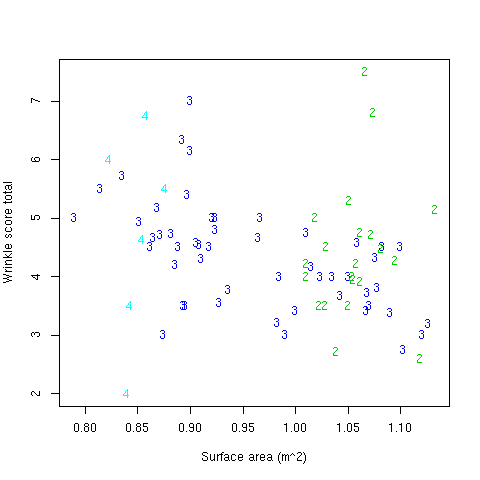
\includegraphics[width=0.9\textwidth]{sawrt.png}
  \caption{Plot of sire group means  of urface area $(m^{2})$ against total wrinkle score (WrT). The numbers representing each point are $Np$.}
  \label{fig:sawrt}
\end{figure}

%\end{document}


The correlation of Sarea with WrT is -0.30, significant at $P<0.05$. The number labels on the points again represt $N_{p}$, and this time there is a pattern. THe low $N_{p}$ sheep are high Sarea and low wrinkle. So it is reasonable to conclude that animals with high growth ( of the whole body, and the skin) stretch out their wrinkles which were formed as a lamb, and reduce the wrinkle score. This is probably what happens with British Longwool sheep, which were shown in the previous section to have quite a high $F_{as}$ value, but do not show wrinkle as an adult.

So we need to try and take surface area into account. We note again that $N_{p}$ reflects both overall growth and extra skin expansion dure to secondary follicle development, while $Sarea$  reflects only overall growth. We therefore take the ratio $N_{p}/Sarea$ as an indicator of skin expansion 'corrected for' growth.  Figure~\ref{fig:fasfnpuaovsa} shows that $N_{p}/Sarea$ ratio is indeed correlated with $F_{as}$.
%\documentclass{article}
%\usepackage{graphicx,subfigure}
%\begin{document}

\begin{figure}[!h]
  \centering
   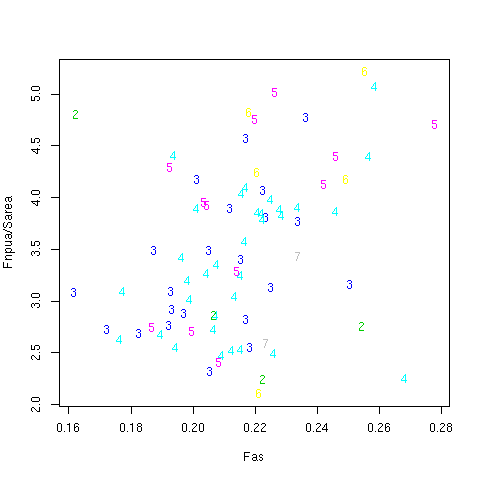
\includegraphics[width=0.9\textwidth]{fasfnpuaovsa.png}
  \caption{Plot of sire group means  of secondary follicle tissue per $mm^{2}$ against the ratio $N_{p}/Sarea$. The numbers representing each point are $WrT$.}
  \label{fig:fasfnpuaovsa}
\end{figure}

%\end{document}


The correlation is 0.33 which is significant at $P<0.01$.  The point labels show a tendency for high wrinkle scores to occur at high $F_{as}$ as observed in Figure~\ref{fig:faswrt}. There is no obvious relation of wrinkle score to $N_{p}/Sarea$ ratio. 

The end point for this dataset is that we think we can measure the extra dermal expansion due to secondary follicle development, but it does not necessarily relate strongly to wrinkle scores, because wrinkle also depends on collagen development. There is no measure of collagen in this dataset, so that is about as far as we can proceed.

\subsection{Rex mutation}
It was noted in Jackson(2017)~\cite{jack:17c} that there was a substantial jump is S/P ratio during evolution of the Finewool Merino, and that this jump may have been produced by mutation at the Rex locus. In other species (cats, rodents) Rex mutation produces a high S/P ratio and a fine coat with no guard hairs and crimp waves in the fibres. 

The other substantial difference between Australian Merinos and other breeds is wrinkle. It is not known when wrinkle appeared in Merino evolution. It is not documented whether Rex mutation in other species produces wrinkle. We thought we would have a look. By googling pictures in Rex mutant cats we uncovered the images shown in Figure~\ref{fig:crex} of a Cornish Rex cat, and the image shown in Figure~\ref{fig:drex} of a Devon Rex cat.
%\documentclass{article}
%\usepackage{graphicx,subfigure}
%\begin{document}

\begin{figure}[!h]
  \centering
   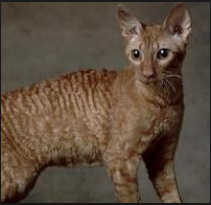
\includegraphics[width=0.9\textwidth]{crex.png}
  \caption{Image if a Cornish Rex cat obtained from Google. This image may be copyright}
  \label{fig:crex}
\end{figure}

%\end{document}


%\documentclass{article}
%\usepackage{graphicx,subfigure}
%\begin{document}

\begin{figure}[!h]
  \centering
   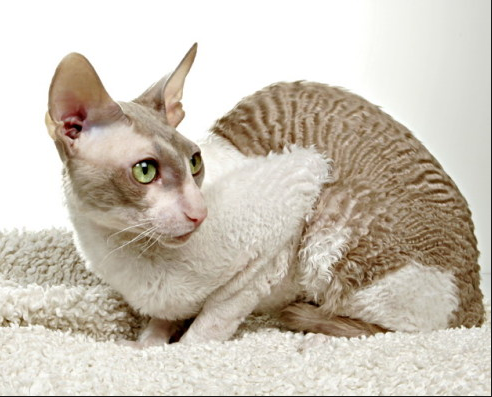
\includegraphics[width=0.9\textwidth]{drex.png}
  \caption{Image if a Devon Rex cat obtained from Google. This image may be copyright}
  \label{fig:drex}
\end{figure}

%\end{document}


We think the wrinkles are obvious. The Devon Rex also shows the wavy fibres clearly.

A similar search of Rex mutant rats and mice uncovered some images of rodents which were both Rex and Naked mutants, and in these the skin wrinkles were obvious. The wrinkles could not be seen on rodents with fur. A search of Rex mutant rabbits did not uncover any visually obvious wrinkle, but all the rabbits had long fur. A discussion with a rabbit breeder confirmed that some Rex rabbits do have skin wrinkles. 

So it would seem that what is going on in Rex mutant cats and rodents is quite similar to what happens in Merino sheep. All Rex mutants have the follicle development to produce excessive dermal expansion, and where there is collagen binding the skin layers this leads to wrinkles, while where there is loose skin ( less collagen binding) wrinkles do not develop. The Merino sheep is just another case.

\subsection{How much dermal expansion is required to form a fold?}
We need to try and calculate whether a dermal expansion of up to 30 percent over the subdermal layers, as estimated in Section~\ref{sec:breed}, is sufficient for the dermal layer to form a fold. We do this with a simple physical model. 

Figure~\ref{fig:model1} shows a piece of leather clamped to a board at two points 50m  apart. 
%\documentclass{article}
%\usepackage{graphicx,subfigure}
%\begin{document}

\begin{figure}[!h]
  \centering
   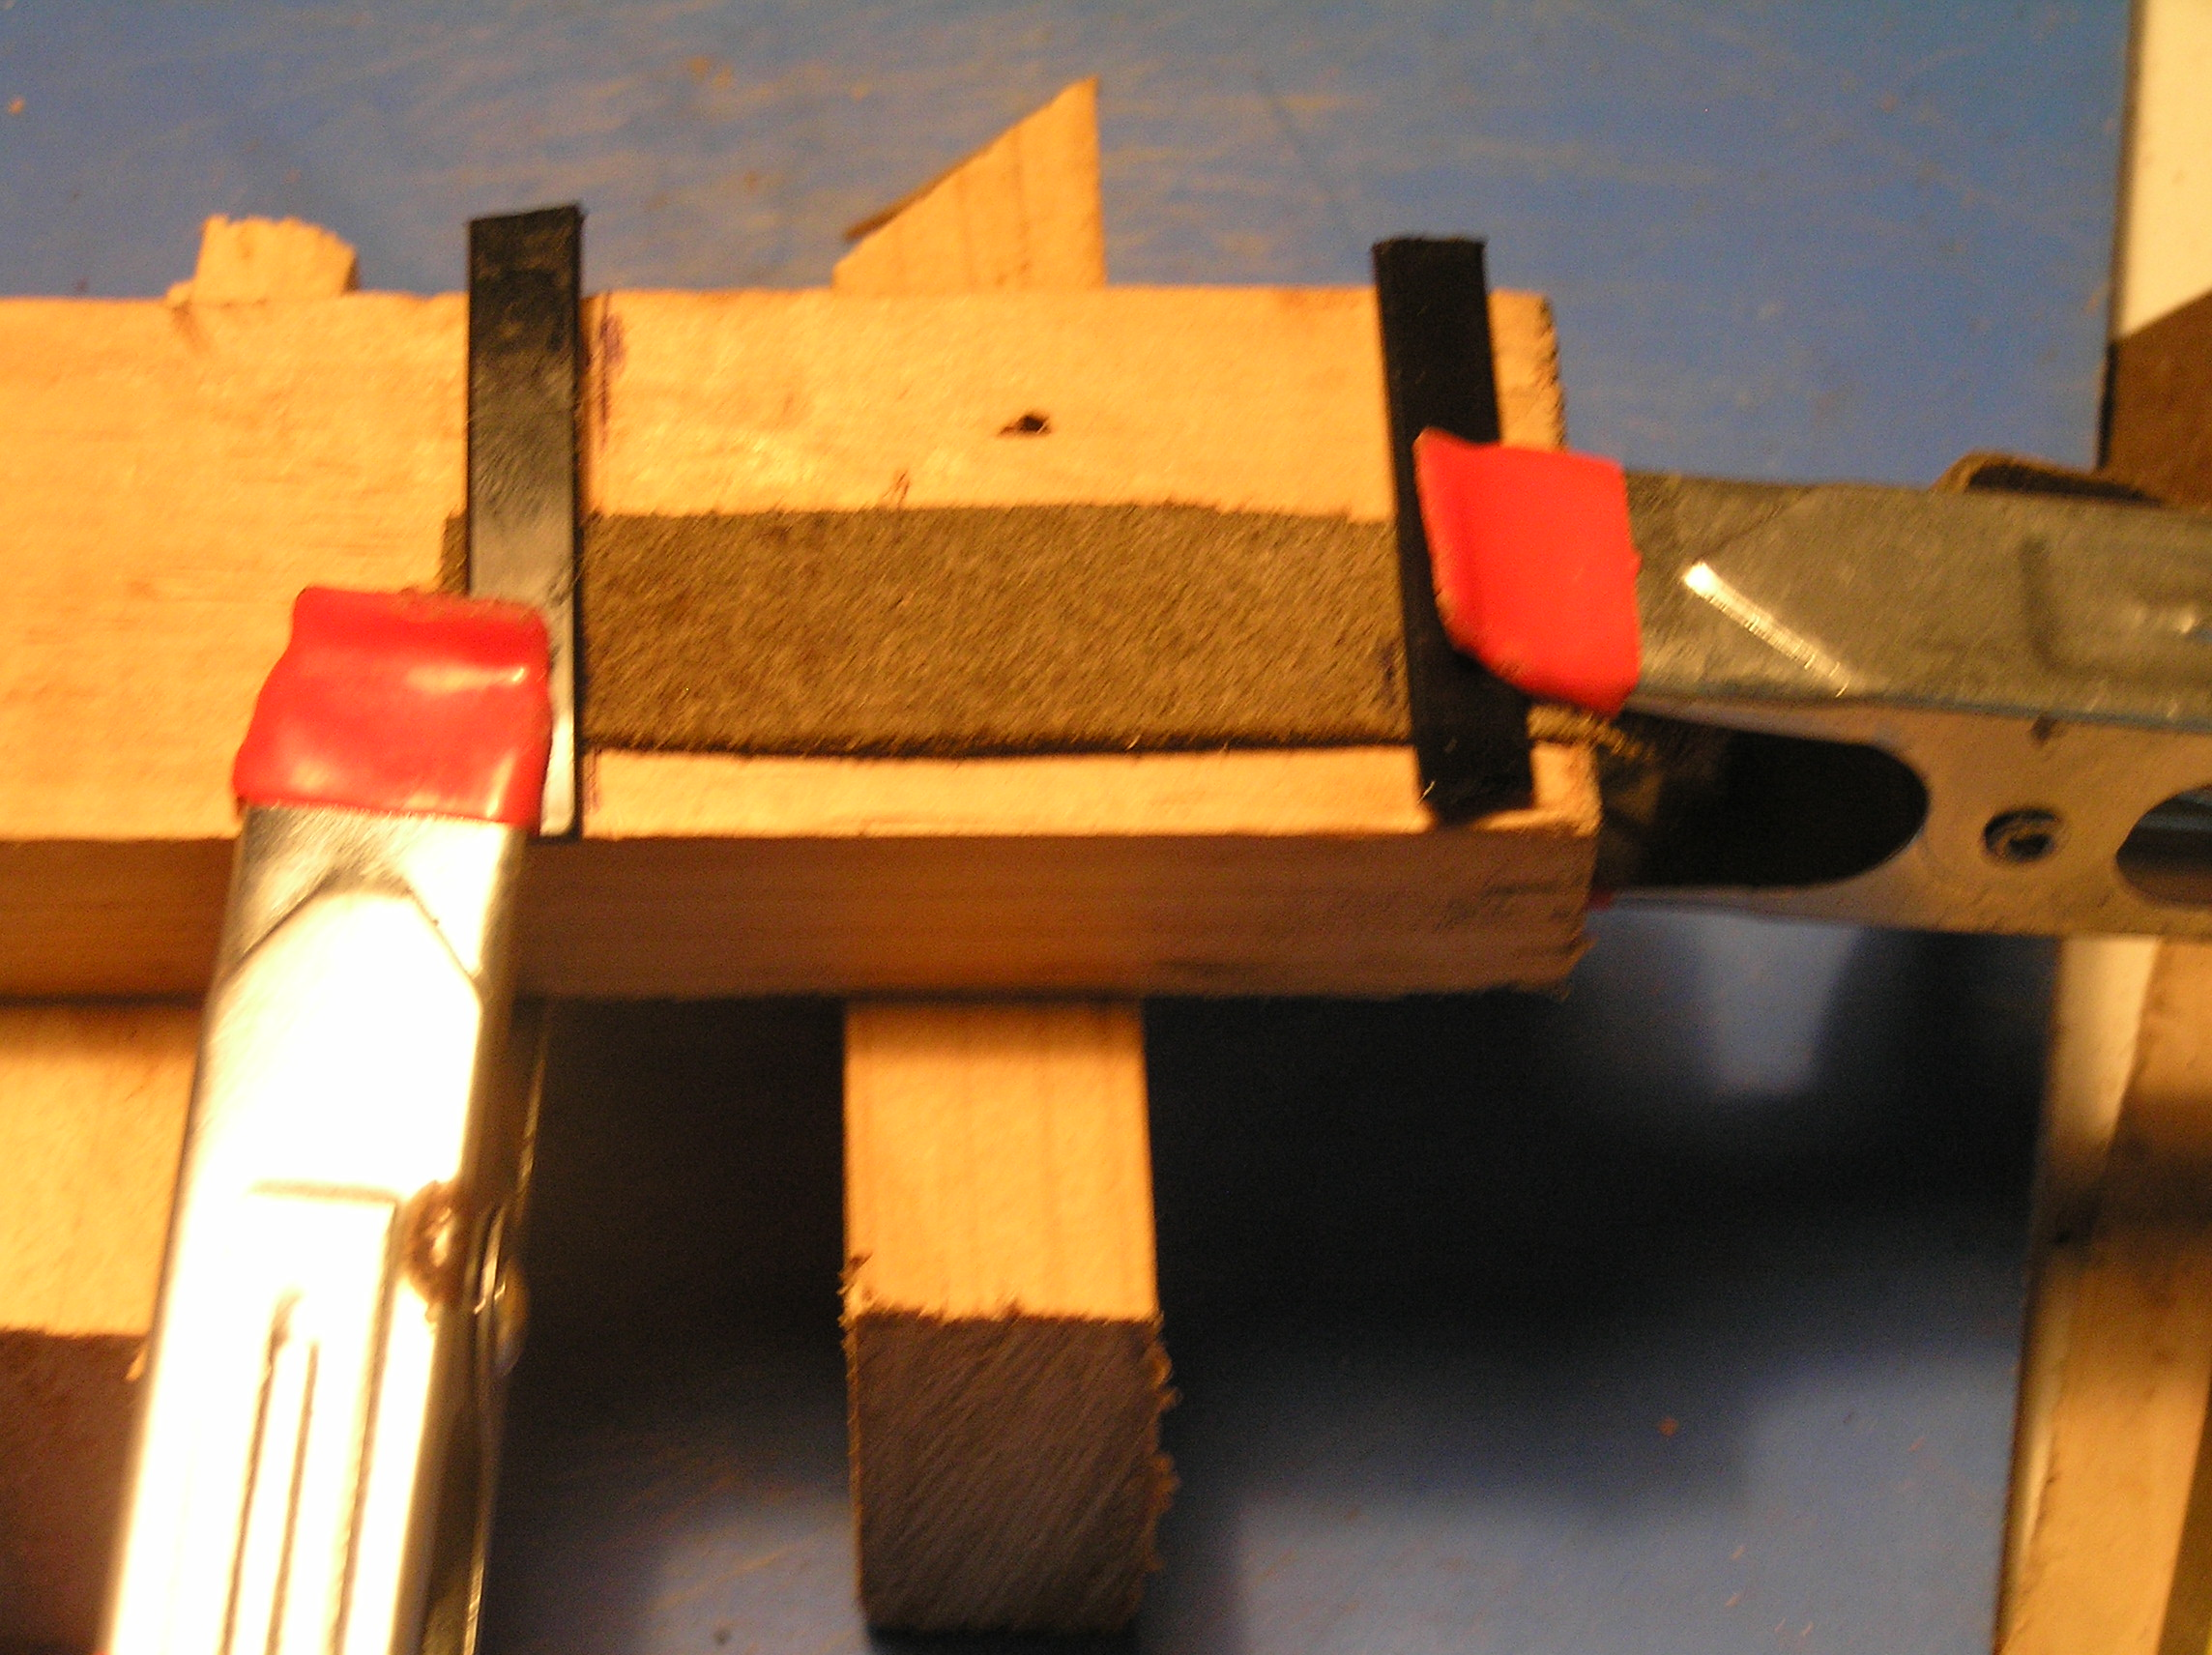
\includegraphics[width=0.9\textwidth]{images/P1010001.JPG}
  \caption{Physical model with a 50mm strip of leather clamped at 0mm and 50mm to a board. The leather represents dermis. The board represents subdermal tissue. This is the starting position with the leather strip clamped at 50mm representing zero dermal expansion}
  \label{fig:model1}
\end{figure}

%\end{document}


The leather represents dermis, the board subdermal tissue. In this case the leather is clamped at 0 and 50mm representing collagen fibres linking the two layers at these two points. However because the leather segment ( 50mm) is the same as the board clamp distance, the leather lies flat, and there is no fold formed. 

If we now increase the leather segment length to 60 mm, and clamp to the board at 50 mm, the leather forms a fold as in Figure~\ref{fig:model2} and Figure~\ref{fig:model3}
%\documentclass{article}
%\usepackage{graphicx,subfigure}
%\begin{document}

\begin{figure}[!h]
  \centering
   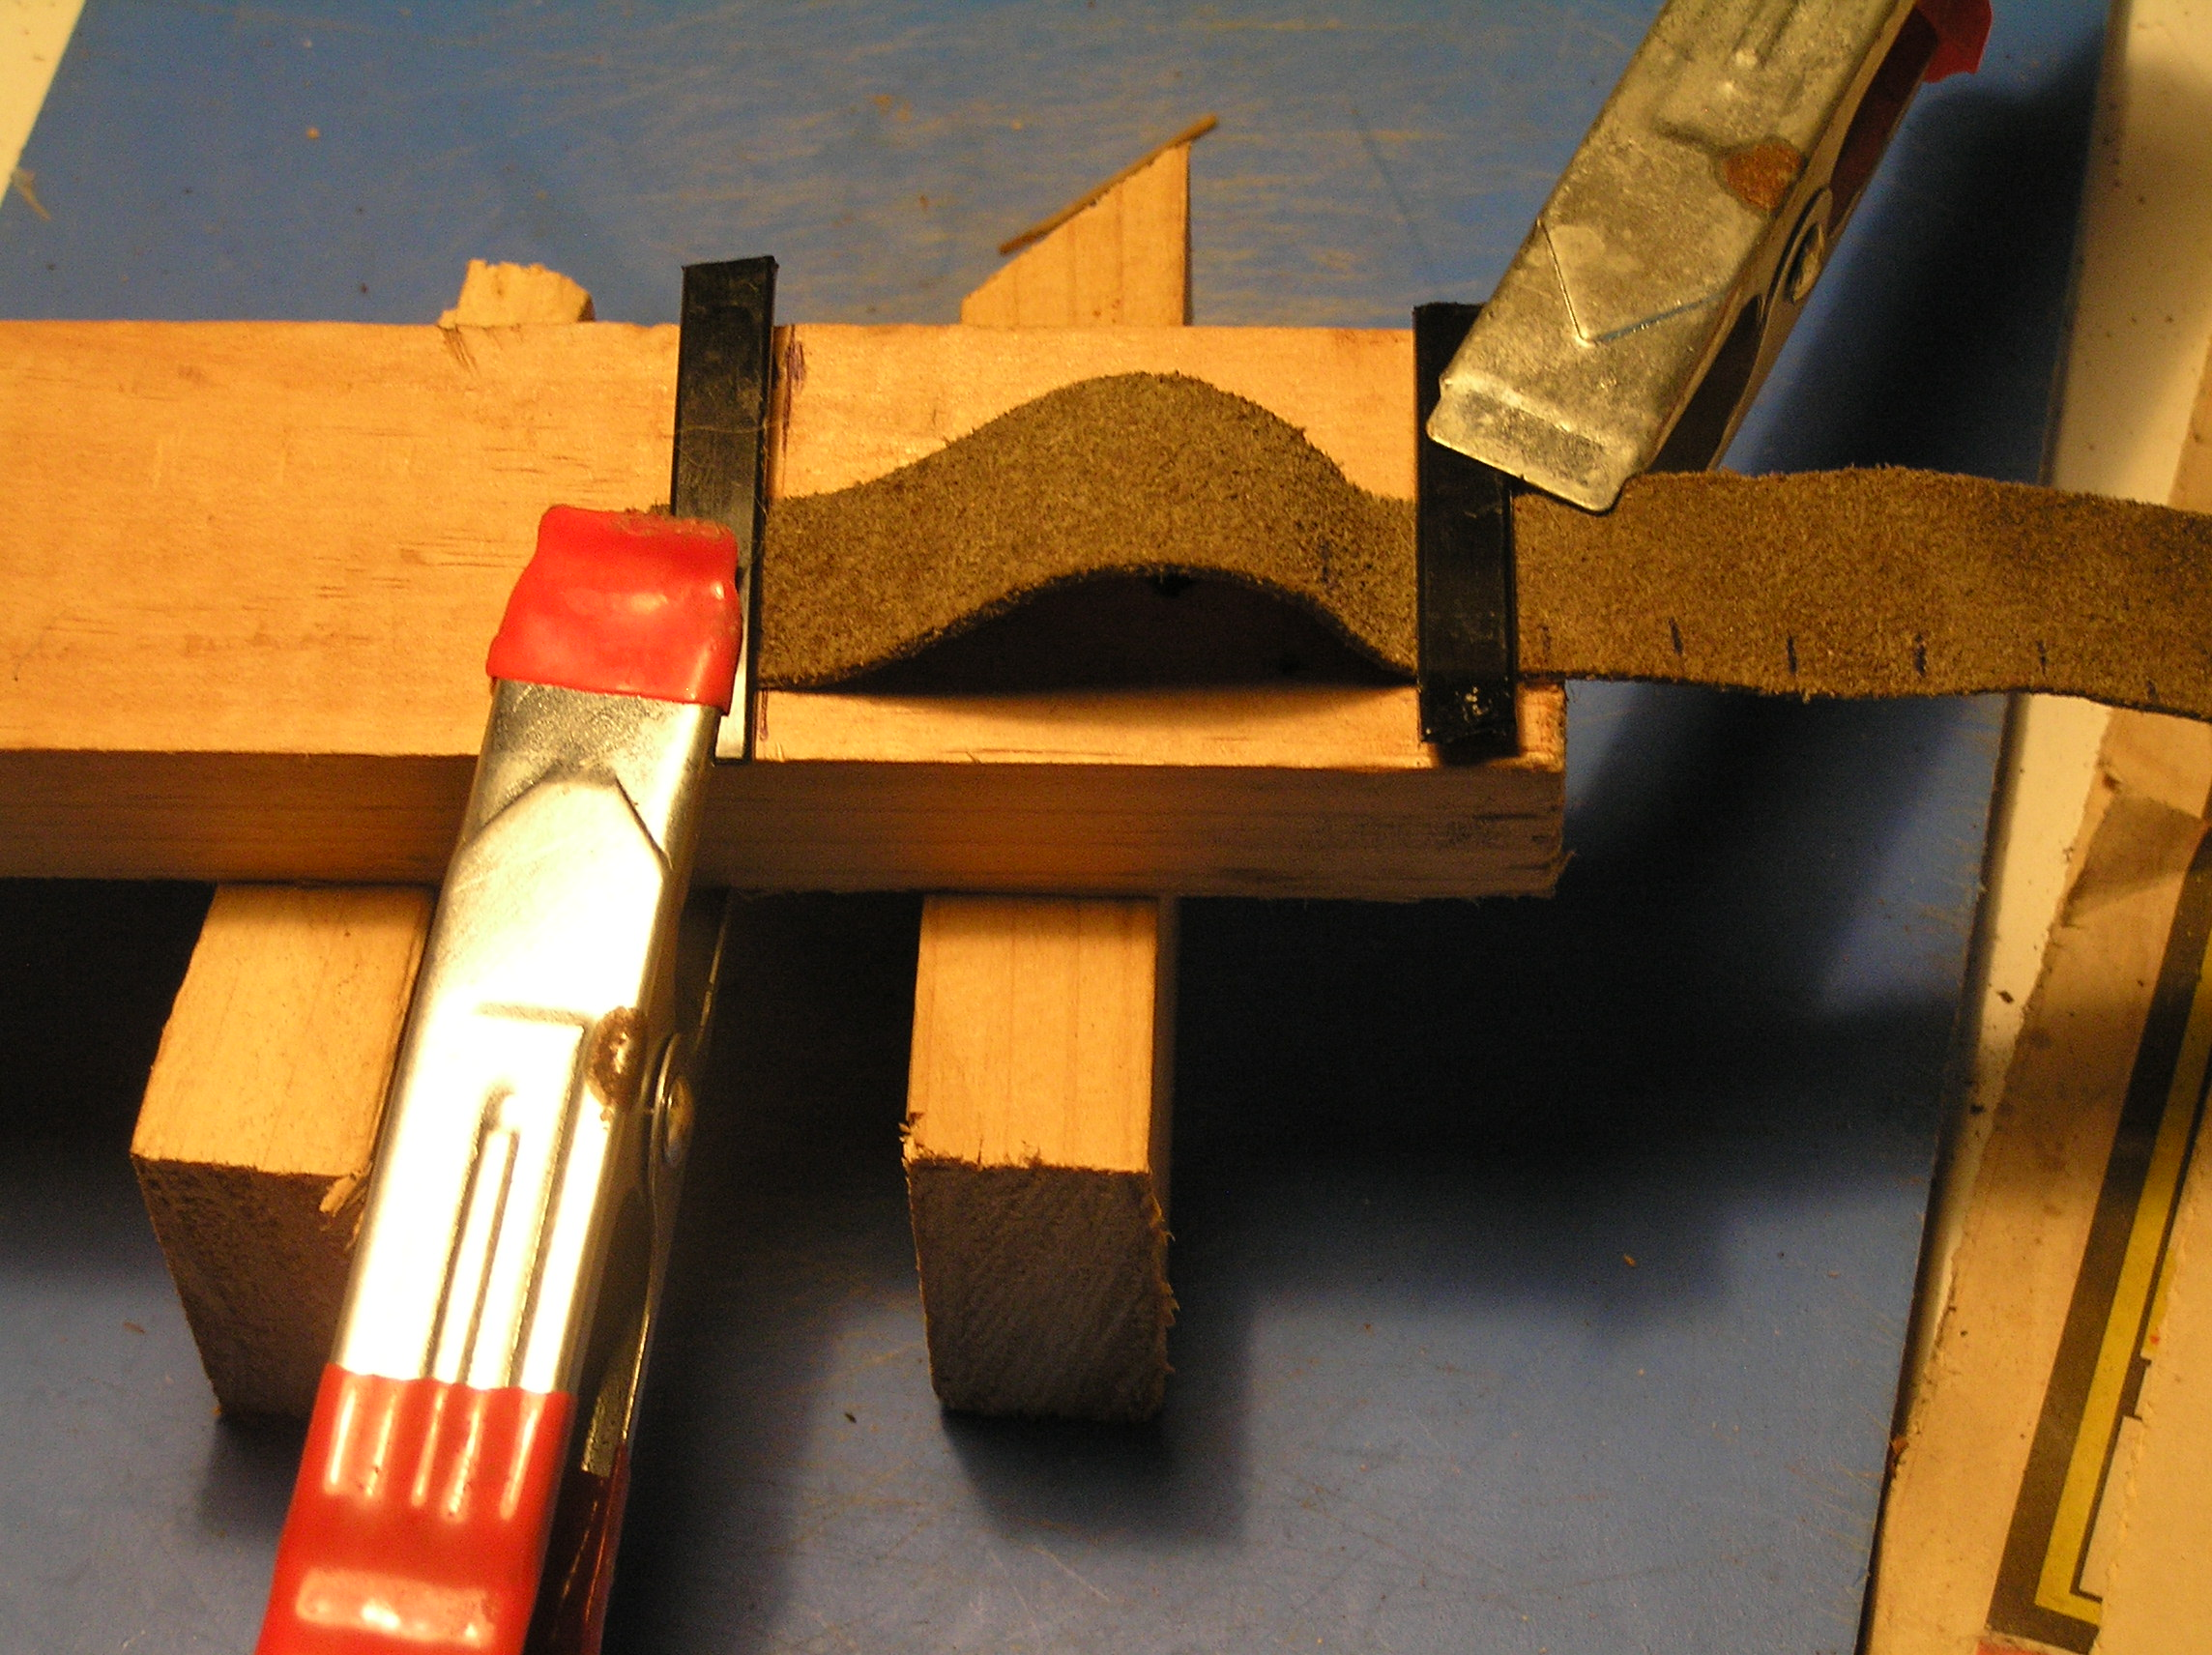
\includegraphics[width=0.9\textwidth]{images/P1010004.JPG}
  \caption{Physical model with a 50mm strip of leather clamped at 0mm and 60mm to a board at positions 0mm and 50mm. The leather represents dermis. The board represents subdermal tissue. This demonstrates fold formation when the leather strip has 10mm of expansion (over the original 50mm), a 20 percent expansion.}
  \label{fig:model2}
\end{figure}

%\end{document}


%\documentclass{article}
%\usepackage{graphicx,subfigure}
%\begin{document}

\begin{figure}[!h]
  \centering
   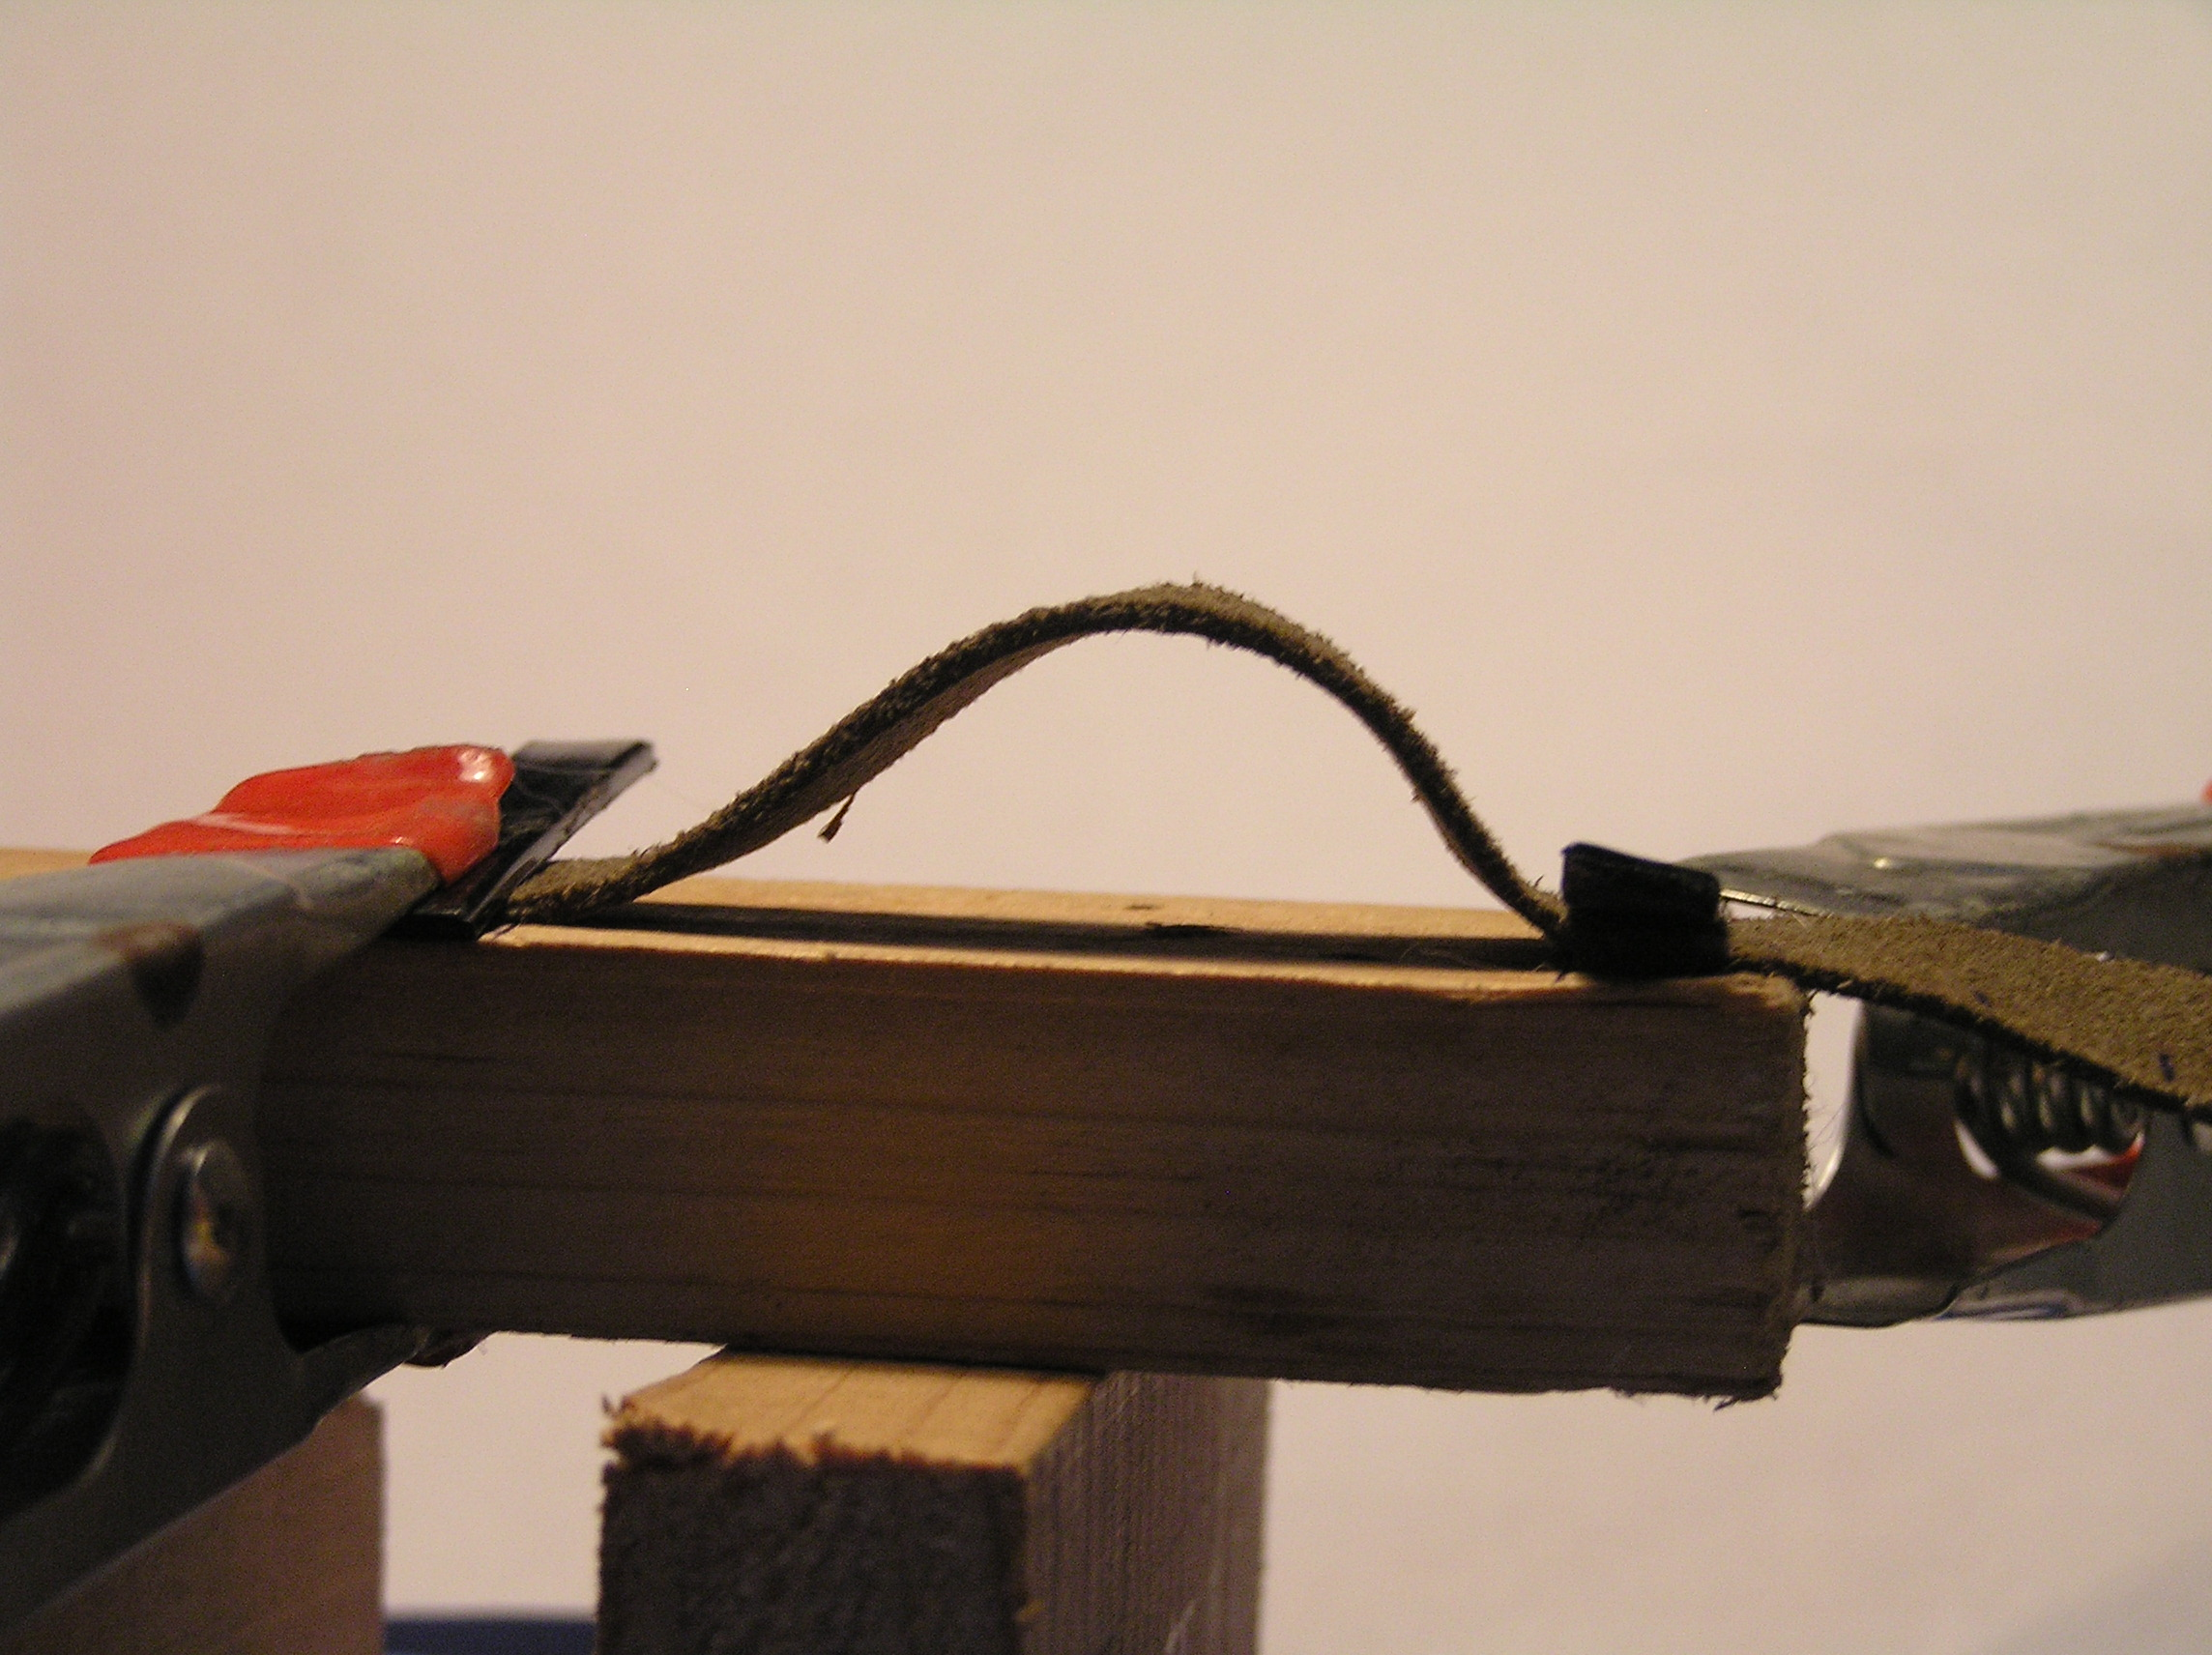
\includegraphics[width=0.9\textwidth]{images/P1010005.JPG}
  \caption{Physical model with a 50mm strip of leather clamped at 0mm and 60mm to a board at positions 0 and 50mm. The leather represents dermis. The board represents subdermal tissue. This demonstrates fold formation when the leather str
ip has 10mm of expansion (over the original 50mm), a 20 percent expansion.}
  \label{fig:model3}
\end{figure}

%\end{document}


We see that there is considerable fold formation with a 20 percent linear expansion of the leather over the board. The measured height of this fold was 16mm.

This model is much larger than real sheepskin. About 10x larger. So if we divide all the results by 10, we are talking about 2 collagen attachment points of dermis to subdermis 5mm apart, a dermal expanded length of 6mm ( or 20 percent larger than subdermis), and the resulting fold being 1.6mm high. That is realistic, but folds on sheep are larger than that. 

So, what specifications are required to get larger folds? We did this with the physical model, using distances between 'collagen attachments' of 30mm, 50mm, and 70mm in the model, corresponding approximately to 3, 5, and 7mm in real skin. For each of these we allowed the leather stip to be clamped at a range of mm (30 - 80 mm in the 30mm case, 50-120mm in the 50mm case, and 70-120mm in the 70mm case), representing dermal expansions over the range 0 to 1.6. The results are given in Table~\ref{tab:model}
% latex table generated in R 3.4.2 by xtable 1.8-2 package
% Sun Mar  4 19:57:01 2018
\begin{table}[ht]
\centering
\caption{Data from the physical model. Width is distance between clamps. Len is length of leather strip between clamps. Height is height of fold. All measurements are in mm. HovW is ratio of Height to Width. LmWovW is (Len - Width)/Len. LHovW and LLmWovW are natural logarithms of the previous 2 columns}
\label{tab:model}
\begin{tabular}{rrrrrrrr}
  \hline
 & Width & Len & Height & HovW & LmWovW & LHovW & LLmWovW \\ 
  \hline
1 &  50 &  50 &   0 & 0.00 & 0.00 & -Inf & -Inf \\ 
  2 &  50 &  60 &  16 & 0.32 & 0.20 & -1.14 & -1.61 \\ 
  3 &  50 &  70 &  23 & 0.46 & 0.40 & -0.78 & -0.92 \\ 
  4 &  50 &  80 &  29 & 0.58 & 0.60 & -0.54 & -0.51 \\ 
  5 &  50 &  90 &  35 & 0.70 & 0.80 & -0.36 & -0.22 \\ 
  6 &  50 & 100 &  39 & 0.78 & 1.00 & -0.25 & 0.00 \\ 
  7 &  50 & 110 &  43 & 0.86 & 1.20 & -0.15 & 0.18 \\ 
  8 &  50 & 120 &  48 & 0.96 & 1.40 & -0.04 & 0.34 \\ 
  9 &  30 &  30 &   0 & 0.00 & 0.00 & -Inf & -Inf \\ 
  10 &  30 &  40 &  12 & 0.40 & 0.33 & -0.92 & -1.10 \\ 
  11 &  30 &  50 &  18 & 0.60 & 0.67 & -0.51 & -0.41 \\ 
  12 &  30 &  60 &  23 & 0.77 & 1.00 & -0.27 & 0.00 \\ 
  13 &  30 &  70 &  27 & 0.90 & 1.33 & -0.11 & 0.29 \\ 
  14 &  30 &  80 &  32 & 1.07 & 1.67 & 0.06 & 0.51 \\ 
  15 &  70 &  70 &   0 & 0.00 & 0.00 & -Inf & -Inf \\ 
  16 &  70 &  80 &  19 & 0.27 & 0.14 & -1.30 & -1.95 \\ 
  17 &  70 &  90 &  26 & 0.37 & 0.29 & -0.99 & -1.25 \\ 
  18 &  70 & 100 &  33 & 0.47 & 0.43 & -0.75 & -0.85 \\ 
  19 &  70 & 110 &  39 & 0.56 & 0.57 & -0.58 & -0.56 \\ 
  20 &  70 & 120 &  44 & 0.63 & 0.71 & -0.46 & -0.34 \\ 
   \hline
\end{tabular}
\end{table}


 We see that we can get folds up to 48m high ( approx 4.8mm on sheep)  but that this height of fold requires from 70 to 160 percent dermal expansion depending on the clamping width. The wider the clamping width, the less percentage dermal expansion needed to form a given height of fold.

With very large folds, the 'bell shape' becomes more horseshoe shaped. Figure~\ref{fig:model4} shows the fold for a 50mm clamp width and a 120mm leather strip length ( a 140 percent expansion).
%\documentclass{article}
%\usepackage{graphicx,subfigure}
%\begin{document}

\begin{figure}[!h]
  \centering
   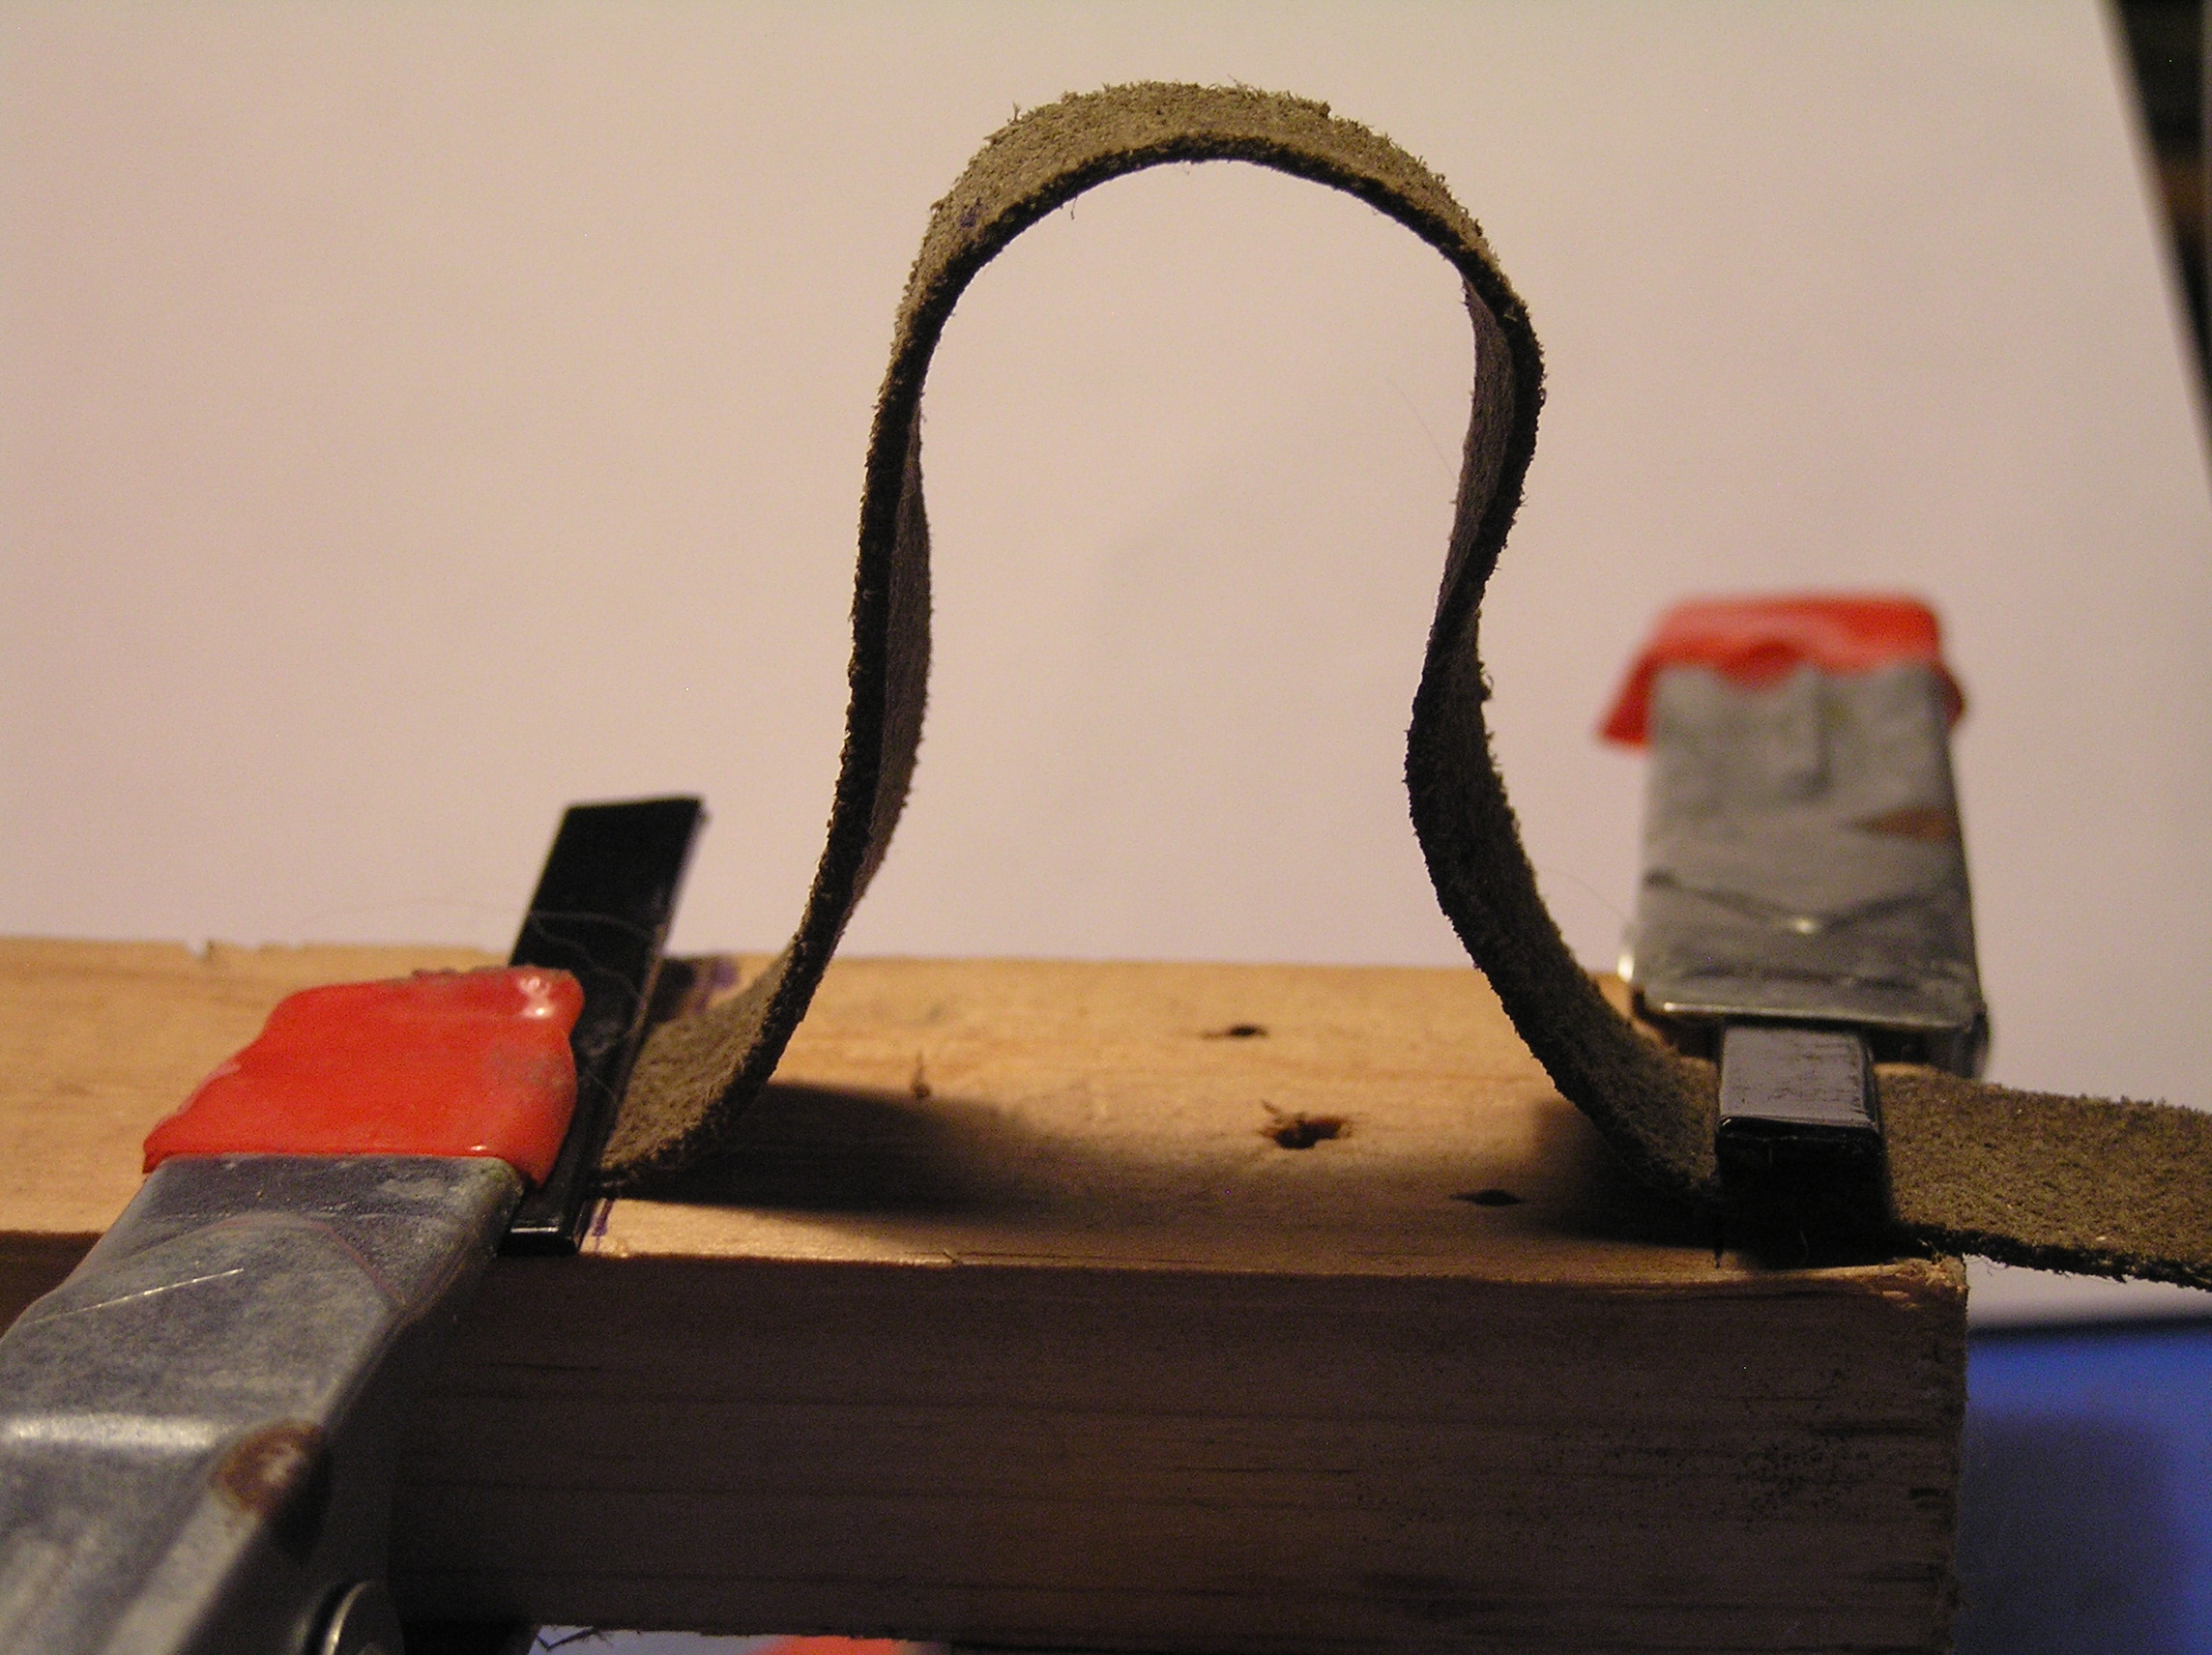
\includegraphics[width=0.9\textwidth]{images/P1010019.JPG}
  \caption{Physical model with a 50mm strip of leather clamped at 0mm and 120 to a board at positions 0 and 50mm. The leather represents dermis. The board represents subdermal tissue. This demonstrates fold formation when the leather strip has 70mm of expansion (over the original 50mm), a 140 percent expansion.}
  \label{fig:model4}
\end{figure}

%\end{document}


This is what we might see in a large neck fold.

We can show that the same 'law of folding' applies regardless of the distance between clamping points. In Figure~\ref{fig:hlplot} we plot all the data points from Table~\ref{tab:model}, showing that the ratio of Height to Width bears the same relation to the relative expansion of the leather strip((Len - Width)/Width) regardless of the clamping width. All points are on the same line.
%\documentclass{article}
%\usepackage{graphicx,subfigure}
%\begin{document}

\begin{figure}[!h]
  \centering
   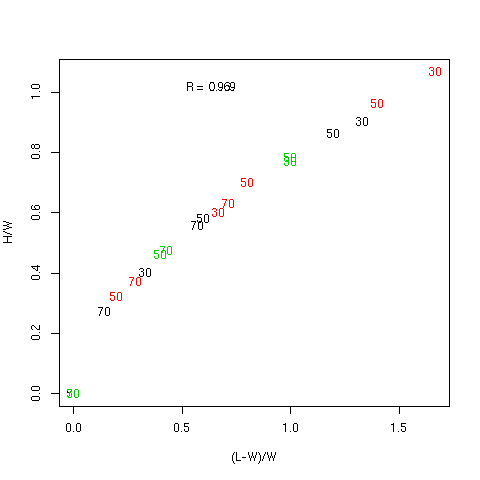
\includegraphics[width=0.9\textwidth]{HLplot.png}
%  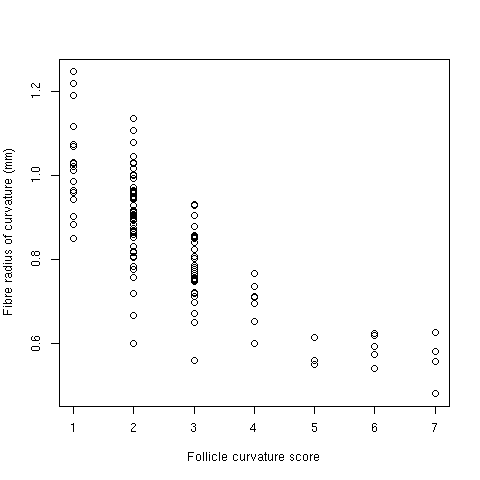
\includegraphics{ofdamm.png}
  \caption{Plot of relative height of each fold against relative expansion of the leather strip against the base clamping length. Each point is represented by its base clamp length.}
  \label{fig:hlplot}
\end{figure}

%\end{document}


 
We can show that this 'law of folding' is a power curve ( of the form $y = aX^{b}$), by doing the log-log plot of the data of Figure~\ref{fig:hlplot}. This is shown in Figure~\ref{fig:loghlplot}.
%\documentclass{article}
%\usepackage{graphicx,subfigure}
%\begin{document}

\begin{figure}[!h]
  \centering
   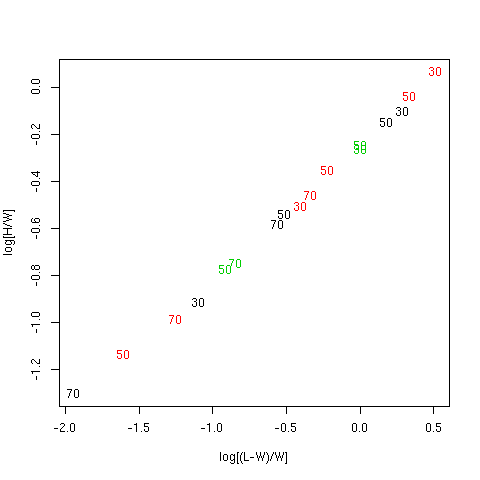
\includegraphics[width=0.9\textwidth]{logHLplot.png}
%  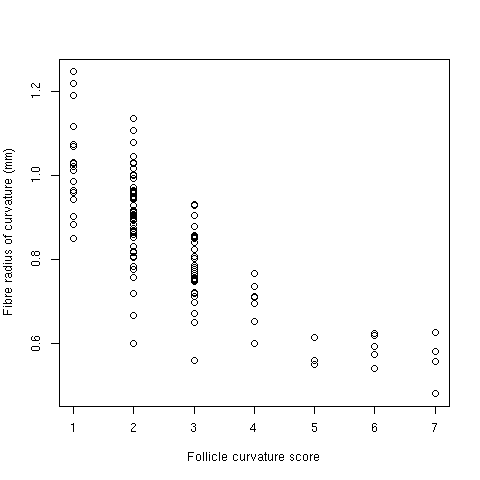
\includegraphics{ofdamm.png}
  \caption{Plot of log relative height of each fold against log relative expansion of the leather strip against the base clamping length. Each point is represented by its base clamp length.}
  \label{fig:loghlplot}
\end{figure}

%\end{document}


We see that the log-log plot is perfectly linear. This proved that it is a power curve.  We can estimate the parameteres of the power curve by fitting a linear regression to the log-log plot ( ie $\log{y} = \log{a} + b \log{x)}$). When we do this we get
\begin{eqnarray*}
\log{a} & = & -0.246 \\
b & = & 0.564
\end{eqnarray*}
 So the power curve is
\begin{displaymath}
\frac{H}{W} = 0.774 \left[\frac{L-W}{W}\right]^{0.564}
\end{displaymath}
 This was done at the scale of the model, but it applies to all scales, so it should be right for real sheepskin, provided the model is appropriate. One factor which should be mentioned is that the model has 'air' under the leather strip, in sheepskin this space is filled with dermal tissue. That may not make a great deal of difference. Most of the dermal expansion is at the epidermal edge of the dermis.

The conclusion from the model and calculations seems to be that a 20  to 30 percent linear expansion due to secondary follicle development will make small folds, but not large folds. We need to qualify this. The 20 to 30 percent estimate of dermal expansion due to follicle development was calculated in Section~\ref{sec:breed} from amount of follicle tissue alone. It did not include accessory glands ( sebacious and sweat glands) or other support tissues ( such as blood vessels). We have no idea how much extra expansion these tissues might lead to, but it is probably at least as much again as the follicle tissue. So our 30 percent upper limit might become 60 percent. So, on the scale of real sheep skin, a 5mm spacing between collagen attachments might lead to a 3mm high wrinkle at the limit. This is more realistic, but still small. Some other factor leading to dermal expansion is required to get large 'neck' folds.  We do show that wider spacing of the collagen 'clamping' points leads to larger wrinkles.

We should note that the model calculates linear expansion - ie in one direction. This is probably what happens. The rows of follicle groups grow like a 'wedge' into the dermis, and drive it 'sideways' rather than in all directions. So when we say that secondary follicle development leads to $0.2 mm^{2}$ per $mm^{2}$ of dermis, we are thinking of a 1mm by 1mm square of dermis becoming a 1mm by 1.2mm rectangle of dermis after secondary follicle development. This is in line with what happens on the sheep. The folds are very definately in one dimension.

\clearpage
\section{Discussion}
We have made a case for development of secondary follicles to be at least partly if not wholly responsible for expansion of the dermal skin layer over and above the normal growth of the subdermal layers, and for this dermal expansion to lead to skin folding or wrinkling, if there are strong collagen attachments between the dermal and subdermal layers.

We have seen that species with a high number of secondary derived follicles ( high S/P ratio) such as Merino sheeep and Rex mutant cats and rodents, sometimes exhibit skin wrinkling. For wrinkles to occur there must be both dermal expansion and collagen cross linking between dermis and lower layers.

 Our vision of dermal expansion is of rows of follicle groups growing down into the dermis and pushing the dermal tissue aside, like a wedge. This is essentially a 1-dimensional effect. Folds are a 1-dimensional phenomenon. Folds form in the same direction down the body of the sheep from dorsal to ventral, as the rows of follicle groups. The correspondence in pattern over the body between folds and follicle groups is remarkable.

For a fold to form, the dermal and subdermal layers must be bound together at some points, and not bound in between these points. The relative height of a fold depends on the 1-dimensional expansion of the dermis relative to the distance between binding points.  It is a simple power curve relationship.

Data such as wrinkle scores on sheep are difficult to interpret.  Scores tend to be affected by body size. Wrinkly sheep do tend to have more secondary follicle tissue, but the correlation is only moderate. Wrinkly sheep also tend to have high follicle curvature and disrupted follicle groups, suggesting that the presence of a lot of collagen interferes with follicle development. It has been observed ( Williams ref?)  that follicles on a wrinkle are less curved than follicles on a flat area between wrinkles. This suggests that there is less collagen at a wrinkle than at the flat points between wrinkle. That is what our model of fold formation assumes. We need to confirm this, because it contradicts the 'popular view' that wrinkles are collagen-rich.

One way of getting a confirmation, is {\em by exclusion}. What do we get when there is a low S/P ratio, only a small contribution of secondary follicle development to dermal expansion, and presumably insufficient dermal expansion for wrinkle development? Well, let us look at British Downs-wool sheep breeds. These have low S/P ratio, presumably few Sd follicles, so there is nothing driving dermal expansion. However they do have a high development of collagen, leading to high follicle curvature, disrupted follicle groups, and poor fibre alignment in the staple, and a low fibre length growth rate. So what is the skin like? It is flat ( not wrinkled) but it is 'tight' not 'loose', indicating that there is collagen binding at all points along the dermis/subdermal border. This proves that dermal expansion (presumably from secondary follicle development) is a requirement for wrinkles to form. Collagen development alone, will not do it.

In saying that follicle development contributes to wrinkle formation, we are not saying that secondary follicle development is undesirable. It is highly desirable. High S/P individuals are among the most productive types, provided they do not develop wrinkle. The key issue is that wrinkle development in high S/P individuals can be avoided by having less collagen development, so that the dermis is not rigidly bound to the subdermal layers at any point and can expand any amount like one giant fold encompassing the whole body. That is the principle behind development of the SRS Merino. The Merino industry in Australia, in particular, needs a new path forward, and this is at least one viable option.

Much of what we say here needs to be verified. That work is in progress.




\clearpage
\begin{thebibliography}{99}

\bibitem{bogo:40}
 Bogolyubsky S.N. (1940) cited by Fraser A.S and Short B.F. (1960) The Biology of the Fleece. Animal Research Laboratories Technical Paper No 3. CSIRO Melbourne 1960.

\bibitem{brow:68}
Brown, G.H., and Turner, Helen Newton. (1968) Response to selection in Australian Merino sheep. II. Estimates of phenotypic and genetic parameters for some production traits in Merino ewes and an analysis of the possible effects of selection on them. Aust. J. Agric. Res. 19:303-22

\bibitem{cart:43}
Carter H.B. (1943) Studies in the biology of the skin and fleece of sheep. 1. The development and general histology of the follicle group in the skin of the Merino. 2. The use of tanned sheepskin in the study of follicle population density. 3. Notes on the arrangement, nomenclature, and variation of skin folds and wrinkles in the Merino. C.S.I.R. Bulletin No 164, Melbourne, 1943

\bibitem{cart:68}
Carter,H.B. (1968) Comparative Fleece Analysis Data for Domestic Sheep. The Principal Fleece Staple Values of Some Recognised Breeds. Agricultural Research Council, 1968

\bibitem{fras:60}
Fraser A.S and Short B.F. (1960) The Biology of the Fleece. Animal Research Laboratories Technical Paper No 3. CSIRO Melbourne 1960.

\bibitem{gord:08}
Gordon-Thompson, C., Botto, S.A., Cam, G.R., and Moore, G.P.H. (2008) Notch pathway gene expression and wool follicle cell fates. Aust. J. Exp. Agric. 48(5) 648-656

\bibitem{jack:75}
Jackson, N., Nay, T, and Turner, Helen Newton (1975) Response to selection in Australian Merino sheep. VII Phenotypic and genetic parameters for some wool follicle characteristics and their correlation with wool and body traits. Aust. J. Agric. Res. 26:937-57

\bibitem{jack:15}
Jackson, N. (2015) Genetic relationship betweeen skin and wool traits in Merino sheep. Incomplete manuscript.

\bibitem{jack:17}
Jackson, N. (2017) Genetics of primary and secondary fibre diameters and densities in Merino sheep. URL https://github.com/nevillejackson/atavistic-sheep/mev-rewrite/supplementary/genetic-parameters/psparam.pdf

\bibitem{jack:17a}
Jackson, N. (2017) Genetic relationship between skin and wool traits in Merino sheep. Part I Responses to selection and estimates of genetic parameters. URL https://github.com/nevillejackson/Fleece-genetics/tree/master/skinandfleeceparameters/ab3220/skinwool1.pdf

\bibitem{jack:17c}
Jackson, N. (2017) What are the defining characteristics of a primitive sheep relative to a modern Merino sheep? URL https://github.com/nevillejackson/atavistic-sheep/mev-rewrite/suppelementary/primitive/primitive.pdf

\bibitem{jack:90}
Jackson, N., Maddocks, I.G., Lax, J., Moore, G.P.M. and Watts, J.E. (1990) Merino Evolution, Skin Characteristics, and Fleece Quality. URL https://github.com/nevillejackson/atavistic-sheep/mev/evol.pdf 

\bibitem{jack:17b}
Jackson, N. and Watts, J.E. (2017) What is known about the genetics of wrinkle score in Merino sheep? URL https://github.com/nevillejackson/Fleece-genetics/wrinkle/wrinkle.pdf

\bibitem{knig:93}
Knight, K.R., Lepore, D.A., Horne, R.S., Ritz, M., Kumta, S. and O'Brian, B.M. (1993) Collagen content of uninjured skin and scar tissue in foetal and adult sheep. Int. J. Exp. Pathol. 74(6):583-591

\bibitem{madd:88}
Maddocks, I.G. and Jackson, N. (1988) Structural studies of sheep, cattle, and goat skin. CSIRO, Division of Aimal Production, Sydney.

\bibitem{ment:80}
Menton, D.N. and Hess, R.A. (1980) The ultrastructure of collagen in the dermis of tight-skin (Tsk) mutant mice. The Journal of Investigative Dermatology 74:139-147

\bibitem{mitc:84}
Mitchell, T.W. et al (1984) Wool Technology and Sheep Breeding, No IV, 200-206

\bibitem{moor:89}
Moore G.P.M., Jackson, N., and Lax, J. (1989) Evidence of a unique developmental mechanism specifying bot wool follicle density and fibre size in sheep selected for single skin and fleece characters. Genet. Res. Camb. 53:57-62

\bibitem{moor:98}
Moore, G.P.M., Jackson, N., Isaacs, K., and Brown, G (1998) J. Theoretical Biology 191:87-94

\bibitem{nay:66}
Nay, T. (1966) Wool follicle arrangement and vascular pattern in the Australian Merino. Aust. J. Agric. Res. 17:797-805

\bibitem{rprog:13}
R Core Team (2013). R: A language and environment for statistical
  computing. R Foundation for Statistical Computing, Vienna, Austria.
  ISBN 3-900051-07-0, URL http://www.R-project.org/.

\bibitem{ryde:68}
Ryder, M.L. and Stevenson, S.K.(1968) Wool Growth. Academic Press, London.


\bibitem{turn:56} 
Turner, Helen Newton (1956) Anim. Breed. Abstr. 24:87-118

\bibitem{turn:58}
Turner, Helen Newton(1958) Aust. J. Agric. Res. 9:521-52

\bibitem{turn:53}
Turner, Helen Newton, Hayman, R.H., Riches, J.H., Roberts, N.F., and Wilson, L.T. (1953) Physical definition of sheep and their fleece for breeding and husbandry studies: with particular reference to Merino sheep. CSIRO Div. Anim. Hlth. Prod. Div. Rept. No. 4 (Ser SW-2 mimeo)

\bibitem{turn:70}
Turner, Helen Newton, Brooker M.G. and Dolling, C.H.S (1970) Response to selection in Australian Merino sheep. III Single character selection for high and low values of wool weight and its components. Aust.J.Agric.Res. 21:955-84

\bibitem{watt:17}
Watts, J.E., Jackson, N., and Ferguson, K.A. (2017) Improvements in fleece weight weight and wool quality of Merino sheep selected visually for high fibre density and length. URL https://github.com/nevillejackson/SRS-Merino/Paper\_2\_Revised\_10\_November\_2017.docx 

\bibitem{watt:17b}
Watts, J.E. and Jackson, N. (2017) Is collagen quantity and properties involved in wrinkle formation and/or in follicle development? URL https://github.com/nevillejackson/SRS-Merino/tree/master/supplementary/copllagen/collagen.pdf

\bibitem{xavi:03}
Xavier, S.P., Gordon-Thomson, C. Wynn, P.C., McCullagh, P., Thomson, P.C., Tomkins, L., Mason, R.S., and Moore, G.P.M.(2003) Evidence that Notch and Delta expressions have a role in dermal condensate aggregation during wool follicle initiation. Experimental Dermatology, 22:656-681

\end{thebibliography}
\end{document}
